\part{Integração das Soluções}

\chapter{Captação de Água}

\section{Parte estrutural}

No Brasil, o sistema para captação de água é utilizado em algumas cidades do Nordeste como fonte de suprimento de água devido aos períodos de seca. A viabilidade do uso de água da chuva é caracterizada pela diminuição da demanda de água fornecida por companhias de saneamento, gerando assim uma economia de custos com a água e redução de retenção da mesma em locais que possam causar enchentes \citep{MAY}.
O principal objetivo da captação e aproveitamento das águas da chuva é: utilização nos banheiros para as descargas de vasos sanitários. Evitando acúmulo de água em locais com depressão, por captar a água e canalizá-la para um reservatório.

\section{Volume de água armazenada}

Antes de aferirmos o volume que devemos armazenar é preciso levar em conta a quantidade de meses no ano em que será possível fazer a captação da água da chuva, o índice de precipitação mensal e a área da superfície que tenha como escoar a água para um reservatório ou vertente: telhados, lajes ou pátios construídos com esta finalidade. 

Como é possível observar na figura 109 que mostra a chuva acumulada mensal no ano de 2011 e compara com a normal climatológica entre 1961 e 1990. Esta normal climatológica para o Distrito Federal indica que no período de outubro a abril são meses mais apropriados para a captação da água da chuva e que no período de maio a setembro são meses bastantes críticos para a captação devido aos baixos índices de precipitação. 

Tendo definido o período de captação e o período de utilização dessa água captada é preciso analisar a índice de precipitação em cada gráfico para cada ano ou utilizar os índices da normal climatológica. Portando esses valores precisa-se ainda determinar a área da superfície coletora da água. No caso do parque urbano e vivencial do gama serão utilizadas as áreas dos telhados do banheiro, guarita, quiosque, sede administrativa e da torre de vigilância como superfície. 

\begin{table}[h]
\centering
\caption{Área dos telhados do parque.}
\label{Área dos telhados do parque.}
\begin{tabular}{lll}
 & \multicolumn{2}{l}{} \\ \hline
\multicolumn{1}{|l|}{Superfície (Telhado)} & \multicolumn{2}{l|}{Área da superfície em $m^{2}$} \\ \hline
\multicolumn{1}{|l|}{Banheiro} & \multicolumn{2}{l|}{43,71 $m^{2}$} \\ \hline
\multicolumn{1}{|l|}{Guarita} & \multicolumn{2}{l|}{23,76 $m^{2}$} \\ \hline
\multicolumn{1}{|l|}{Quiosque} & \multicolumn{2}{l|}{113,17 $m^{2}$} \\ \hline
\multicolumn{1}{|l|}{Sede Administrativa} & \multicolumn{2}{l|}{136 $m^{2}$} \\ \hline
\multicolumn{1}{|l|}{Torre de Vigilância} & \multicolumn{2}{l|}{60,84 $m^{2}$} \\ \hline
\multicolumn{1}{|l|}{TOTAL} & \multicolumn{2}{l|}{377,48 $m^{2}$} \\ \hline
\end{tabular}
\end{table}

Com essas informações: área de captação de água da chuva, índice de precipitação, pode-se calcular quanto de água da chuva seu telhado ou superfície será capaz de coletar. Para calcular, utiliza-se a fórmula \cite{SANEPAR}:

\begin{equation}
V = iA 
\end{equation}


Onde: V = Volume (mensal ou anual),  i = Intensidade de precipitação e A = Área estimada para captação. 

Bastando multiplicar a área do telhado pelos milímetros de chuva indicados nos gráficos, encontra-se o volume. O resultado será sempre em litros. Sendo assim, é possível calcularmos o volume de água nos meses favoráveis a captação, como exemplo, para os anos de 2011-2014 e comparar com a normal climatológica (61-90). A normal climatológica é o valor médio do volume de precipitações correspondente a um número de anos suficiente para se poder admitir que ele representa o valor predominante daquele elemento no local considerado \cite{IPMA}.


\begin{figure}[H]
	 \centering
	\label{Chuva acumulada mensal (2011) x chuva (Normal climatólogia 61-90)}
	 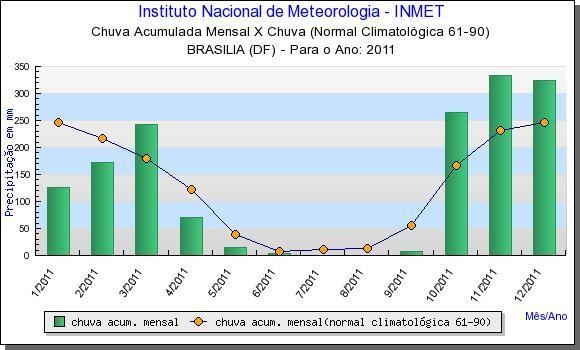
\includegraphics[scale=0.6]{captacao/1.jpg}
	 \caption{Chuva acumulada mensal (2011) x chuva (Normal climatólogia 61-90).}
	 \small{Fonte: \cite{INMET}}
\end{figure}
 
 
\begin{figure}[H]
	 \centering
	\label{Chuva acumulada mensal (2012) x chuva (Normal climatólogia 61-90)}
	 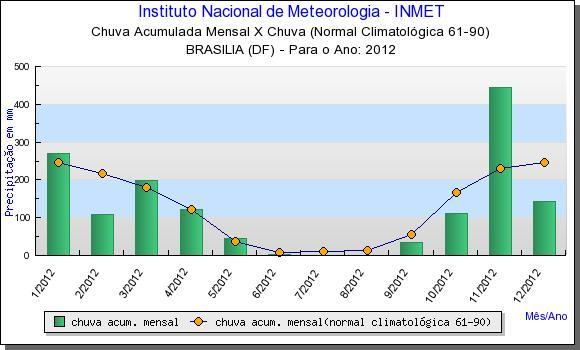
\includegraphics[scale=0.6]{captacao/2.jpg}
	 \caption{Chuva acumulada mensal (2012) x chuva (Normal climatólogia 61-90).}
	\small{Fonte: \cite{INMET}}
\end{figure}

\begin{figure}[H]
	 \centering
	\label{Chuva acumulada mensal (2013) x chuva (Normal climatólogia 61-90)}
	 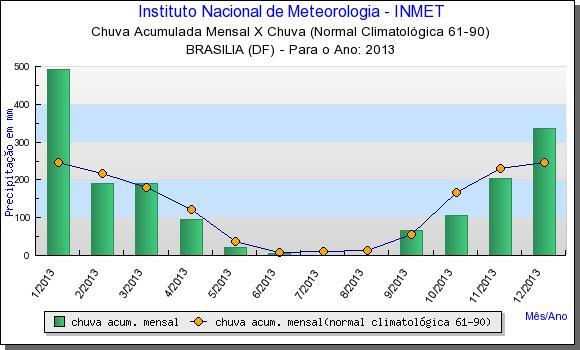
\includegraphics[scale=0.6]{captacao/3.jpg}
	 \caption{Chuva acumulada mensal (2011) x chuva (Normal climatólogia 61-90).}
	\small{Fonte: \cite{INMET}}
\end{figure}
 
 
\begin{figure}[H]
	 \centering
	\label{Chuva acumulada mensal (2014) x chuva (Normal climatólogia 61-90)}
	 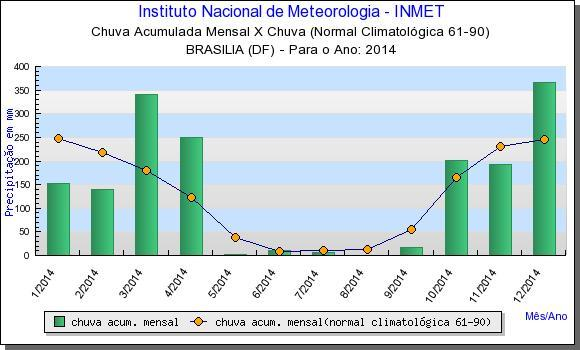
\includegraphics[scale=0.6]{captacao/4.jpg}
	 \caption{Chuva acumulada mensal (2012) x chuva (Normal climatólogia 61-90).}
	\small{Fonte: \cite{INMET}}
\end{figure}

\begin{table}[h]
\centering
\caption{Volume acumulado dos meses favoráveis a captação de água no DF (2011-2014) e (61-90).}
\label{Volume acumulado dos meses favoráveis a captação de água no DF (2011-2014) e (61-90).}
\begin{tabular}{llllll}
 &  &  &  &  &  \\ \hline
\multicolumn{1}{|l|}{} & \multicolumn{5}{l|}{Volume Acumulado em Litros} \\ \hline
\multicolumn{1}{|l|}{Mês} & \multicolumn{1}{l|}{2011} & \multicolumn{1}{l|}{2012} & \multicolumn{1}{l|}{2013} & \multicolumn{1}{l|}{2014} & \multicolumn{1}{l|}{Normal Clim. (61-90)} \\ \hline
\multicolumn{1}{|l|}{Janeiro} & \multicolumn{1}{l|}{49.072} & \multicolumn{1}{l|}{101.919,60} & \multicolumn{1}{l|}{186.852,60} & \multicolumn{1}{l|}{56.622} & \multicolumn{1}{l|}{94.370} \\ \hline
\multicolumn{1}{|l|}{Fevereiro} & \multicolumn{1}{l|}{64.171,60} & \multicolumn{1}{l|}{41.522,80} & \multicolumn{1}{l|}{71.721,20} & \multicolumn{1}{l|}{52.847,20} & \multicolumn{1}{l|}{83.045,60} \\ \hline
\multicolumn{1}{|l|}{Março} & \multicolumn{1}{l|}{90.595,20} & \multicolumn{1}{l|}{75.496} & \multicolumn{1}{l|}{71.721,20} & \multicolumn{1}{l|}{128.343,20} & \multicolumn{1}{l|}{67946,4} \\ \hline
\multicolumn{1}{|l|}{Abril} & \multicolumn{1}{l|}{26.423,60} & \multicolumn{1}{l|}{45.297,60} & \multicolumn{1}{l|}{33.973,20} & \multicolumn{1}{l|}{94.370} & \multicolumn{1}{l|}{49.072,40} \\ \hline
\multicolumn{1}{|l|}{Outubro} & \multicolumn{1}{l|}{101.919,60} & \multicolumn{1}{l|}{37.748} & \multicolumn{1}{l|}{37.748} & \multicolumn{1}{l|}{75.496} & \multicolumn{1}{l|}{64.171,60} \\ \hline
\multicolumn{1}{|l|}{Novembro} & \multicolumn{1}{l|}{124.568,40} & \multicolumn{1}{l|}{166.091,20} & \multicolumn{1}{l|}{75.496} & \multicolumn{1}{l|}{71.721,20} & \multicolumn{1}{l|}{86.820,40} \\ \hline
\multicolumn{1}{|l|}{Dezembro} & \multicolumn{1}{l|}{120.793,60} & \multicolumn{1}{l|}{52.847,20} & \multicolumn{1}{l|}{128.343,20} & \multicolumn{1}{l|}{139.667,60} & \multicolumn{1}{l|}{90.595,20} \\ \hline
\multicolumn{1}{|l|}{TOTAL} & \multicolumn{1}{l|}{577.544} & \multicolumn{1}{l|}{520.922,40} & \multicolumn{1}{l|}{605.855,40} & \multicolumn{1}{l|}{619.067,20} & \multicolumn{1}{l|}{536.021,60} \\ \hline
\end{tabular}
\end{table}

	Após calculado o quanto de água da chuva os telhados do Parque Urbano e Vivencial do Gama coletaram mensalmente e o acumulado para os meses favoráveis a captação da água da chuva no Distrito Federal durante os anos de 2011 e 2014. Agora é preciso determinar o quanto o Parque Urbano e Vivencial do Gama gastará em litros com o uso de descargas e irrigação de jardins.  
	
\section{Uso de descargas}

	Após calculado o quanto de água da chuva os telhados do Parque Urbano e Vivencial do Gama coletaram mensalmente e o acumulado para os meses favoráveis a captação da água da chuva no Distrito Federal durante os anos de 2011 e 2014. Agora é preciso determinar o quanto o Parque Urbano e Vivencial do Gama gastará em litros com o uso de descargas e irrigação de jardins.  
	Espera-se que após o témino das obras no Parque Urbano e Vivencial do Gama o parque receba em torno de 1300 pessoas em dias cheios. Estimando que o parque receba 3000 pessoas por semana e que a descarga dos banheiros sejam utilizadas 1500 vezes e que em cada descarga sejam gastos 6L como no que será utilizado no PUVG - Vaso Sanitário com Caixa Acoplada 3/6L Azálea Branco. Deve-se considerar também que a seca no Distrito Federal dura 5 a 6 meses, portanto a estimativa deve incluí-los. 
	
\begin{table}[h]
\centering
\caption{Consumo total de água em descarga do PUVG nos 6 meses de seca no DF.}
\label{Consumo total de água em descarga do PUVG nos 6 meses de seca no DF.}
\begin{tabular}{lllll}
 &  &  &  &  \\ \hline
\multicolumn{1}{|l|}{Nº descargas/Semana} & \multicolumn{1}{l|}{Litros/Descarga} & \multicolumn{1}{l|}{Dias} & \multicolumn{1}{l|}{Meses} & \multicolumn{1}{l|}{TOTAL em litros} \\ \hline
\multicolumn{1}{|l|}{1500} & \multicolumn{1}{l|}{6} & \multicolumn{1}{l|}{30} & \multicolumn{1}{l|}{6} & \multicolumn{1}{l|}{216.000} \\ \hline
\multicolumn{1}{|l|}{2000} & \multicolumn{1}{l|}{6} & \multicolumn{1}{l|}{30} & \multicolumn{1}{l|}{6} & \multicolumn{1}{l|}{360.000} \\ \hline
\end{tabular}
\end{table}

Portanto, caso em determinado ano a seca se prolongue por 6 meses (normalmente são 5) o parque consumirá de 216.000 L a 360.000 L, quando realizadas 1500 e 2000 descargas por semana respectivamente. 

\section{Quanto eu consigo captar?}

Analisando a tabela 14, especificamente a coluna da Normal Climatológica que revela que o quanto o Parque consegue coletar em litros de água com a superfície de 377,48m2 (área telhados do parque), obtêm-se o valor de 536.021,6L. É baseado nesse valor que se fará o dimensionamento do sistema. Pois a estrutura utilizada para o reservatório (Cement Plate Cistern) comporta até 20 mil litros cada \cite{gnadlinger1999technical}. Logo, seria preciso 27 dessas ou reservatórios maiores ao redor das instalações do parque. No entanto, serão utilizados 8 tanques com capacidade total de 160.000L. Como a água dos reservatórios será utilizada também no período em que está sendo captada e o parque consume mensalmente 60.000L, nem todos os meses a água armazenada será consumida. A tabela abaixo mostra o quanto o parque consegue captar, o volume de água consumida mensalmente (descargas) e o quanto da água captada mensalmente sobraria.

\begin{table}[h]
\centering
\caption{Volume Residual Mensal.}
\label{Volume Residual Mensal.}
\begin{tabular}{lccc}
 & \multicolumn{1}{l}{} & \multicolumn{1}{l}{} & \multicolumn{1}{l}{} \\ \hline
\multicolumn{4}{|c|}{Volume Residual Mensal} \\ \hline
\multicolumn{1}{|l|}{Mês} & \multicolumn{1}{l|}{Volume Captado Mensalmente (Norm. Clim.)} & \multicolumn{1}{l|}{Volume Consumido Mensalmente} & \multicolumn{1}{l|}{Volume Residual em L} \\ \hline
\multicolumn{1}{|l|}{Janeiro} & \multicolumn{1}{c|}{94.370} & \multicolumn{1}{c|}{60.000L} & \multicolumn{1}{c|}{34.370} \\ \hline
\multicolumn{1}{|l|}{Fevereiro} & \multicolumn{1}{c|}{83.045,60} & \multicolumn{1}{c|}{60.000L} & \multicolumn{1}{c|}{23.045,60} \\ \hline
\multicolumn{1}{|l|}{Março} & \multicolumn{1}{c|}{67946,4} & \multicolumn{1}{c|}{60.000L} & \multicolumn{1}{c|}{7.946,40} \\ \hline
\multicolumn{1}{|l|}{Abril} & \multicolumn{1}{c|}{49.072,40} & \multicolumn{1}{c|}{60.000L} & \multicolumn{1}{c|}{-10.927,60} \\ \hline
\multicolumn{1}{|l|}{Outubro} & \multicolumn{1}{c|}{64.171,60} & \multicolumn{1}{c|}{60.000L} & \multicolumn{1}{c|}{4.171,60} \\ \hline
\multicolumn{1}{|l|}{Novembro} & \multicolumn{1}{c|}{86.820,40} & \multicolumn{1}{c|}{60.000L} & \multicolumn{1}{c|}{26.820,40} \\ \hline
\multicolumn{1}{|l|}{Dezembro} & \multicolumn{1}{c|}{90.595,20} & \multicolumn{1}{c|}{60.000L} & \multicolumn{1}{c|}{30.595,20} \\ \hline
\end{tabular}
\end{table}

Como a captação será feita durante sete meses, quando começar o período de estiagem a partir de maio e que segue por cinco meses, o reservatório terá acumulado em água 116.949,2L pois é preciso levar em conta que no mês de abril o volume residual foi negativo. Esse volume residual é quase suficiente para abastecer o parque por mais dois meses, sendo assim durante apenas três o consumo seria suprido pela companhia de abastecimento do Distrito Federal (CAESB).

\section{Processo de captação}

No processo de captação da água, são utilizadas áreas impermeáveis, como por exemplo nos telhados. Este projeto visa a disponibilização da coleta da água nos telhados dos banheiros, da administração e das torres de segurança. Nos locais que tiver certa inclinação, serão colocadas calhas capazes de canalizar a água e levá-la para os tanques, onde serão tratadas e enviadas para sua utilização \cite{MAY}.

Segundo a Leal \cite{LEAL} , o sistema de aproveitamento da água da chuva funciona da seguinte maneira: a água é coletada de áreas impermeáveis e em seguida é filtrada e armazenada em um reservatório de acumulação, que pode ser apoiado, enterrado ou elevado e pode ser construído de diferentes materiais como: concreto armado, bloco de concreto, alvenaria de tijolos, aço, plástico, poliéster, polietileno e outros. 

Os parâmetros principais envolvidos no sistema de coleta e aproveitamento da água de chuva são: área de coleta, quantidade de água a ser armazenada, qualidade da água, capacidade de armazenamento e confiabilidade. 
Para não ocorrerem entupimentos nos dutos que levam a água canalizada para os tanques são usadas peneiras para retirada de folhas e galhos maiores, essas grades serão posicionadas por toda a calha aumentando um pouco o custo, porém evitando possíveis problemas na filtragem, como pode ser observado na Figura 1. Será usado 122mm x 3m dessa calha, e pode ser encontrada na  Leroy Merlin a um valor de R\$ 59,90.

\begin{figure}[H]
	 \centering
	\label{Grades usada na calha.}
	 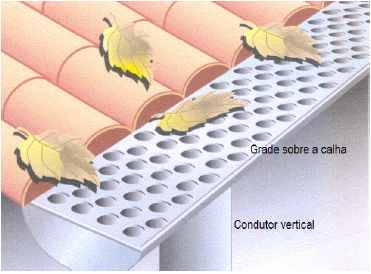
\includegraphics[scale=0.6]{captacao/5.png}
	 \caption{Grades usada na calha.}
	 \small{Fonte: \cite{WATERFALL}}
\end{figure}

\begin{figure}[H]
	 \centering
	\label{Sistema de calhas na área do telhado.}
	 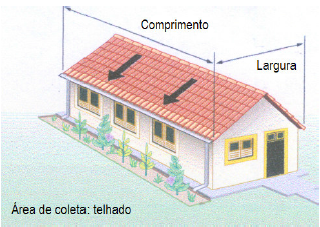
\includegraphics[scale=0.6]{captacao/6.png}
	 \caption{Sistema de calhas na área do telhado.}
	 \small{Fonte: \cite{WATERFALL}}
\end{figure}

O armazenamento será feito a partir do estudo de 8 tipos de tanques, devido a disponibilidade e a facilidade de construção, para tanto foi realizado um estudo, apresentado na Figura 115, da capacidade de armazenamento, viabilidade econÎmica, e mão-de-obra.

\begin{figure}[H]
	 \centering
	\label{Tipo de Tanques}
	 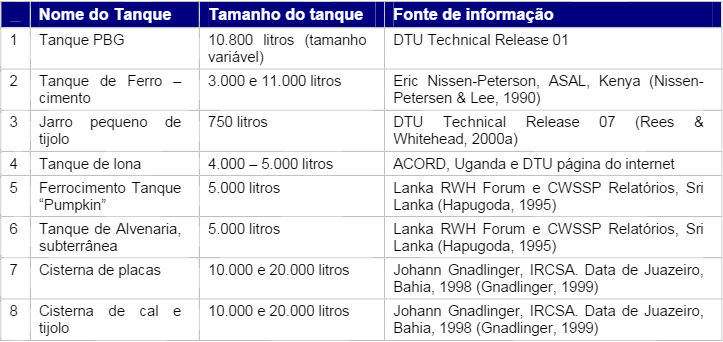
\includegraphics[scale=0.6]{captacao/7.png}
	 \caption{Tipo de Tanques.}
	 \small{Fonte: \cite{gnadlinger1999technical}}
\end{figure}

\begin{figure}[H]
	 \centering
	\label{Comparativo dos tanques}
	 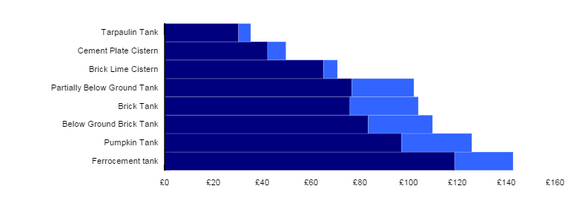
\includegraphics[scale=0.6]{captacao/8.png}
	 \caption{Comparativo dos tanques.}
	\small{Fonte: \cite{gnadlinger1999technical}}
\end{figure}

O gráfico da figura 116 foi feito a partir das informções da Figura 115 sobre os tipos de tanques, mostrando o custo do material, a conversão foi feita seguindo a cotação atual, sendo 1 libra esterlina 4,36 reais.

Tendo em vista os tanques estudados na e apresentados na Figura 115, o que se mostrou mais economicamente atrativo foi o “Cement Plate Cistern”, a cisterna de placas cimentadas, a qual armazena de 10 mil a 20 mil litros de água, o mesmo é melhor para o parque devido ao seu custo de operação e instalação serem baixos, o cimento é barato, gerando um custo de 500 reais para a construção. O tanque do tipo placas cimentadas segue a ideia de ser encostado na edificação, portanto eles serão posicionados ao lado dos banheiros, guarita de segurança, administração e quiosque sem consumir muito espaço e com sinalização para que os usuários não mexam na instalação. A Figura 117 apresenta o sistema de captação de água a ser implantado no Parque do Gama \cite{gnadlinger1999technical}. 

\begin{figure}[H]
	 \centering
	\label{sistema de captação}
	 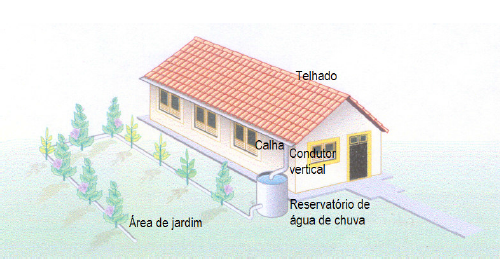
\includegraphics[scale=0.6]{captacao/9.png}
	 \caption{sistema de captação.}
	  \small{Fonte: \cite{WATERFALL}}
\end{figure}

Um ponto relevante a ser considerado é que em hipótese alguma a água de chuva captada poderá ser misturada a água potável. Ademais, é necessário que haja limpeza da água. Para realizar a limpeza da água, será usado um filtro VF1 o qual recebe a água da chuva e filtra os galhos e folhas que passaram pela grade das calhas, em seguida, a água da chuva passa por uma tela de malha de 0,26mm que se localiza abaixo das ripas e é direcionada ao reservatório. A frequência da manutenção varia conforme a incidência da sujeira, ocorrendo de 1 a 2 vezes ao ano. O filtro, o qual vai ser utilizado, é mostrado na Figura 119 e pode ser encontrado no valor de 2100 reais. 


\begin{figure}[H]
	 \centering
	\label{Sistema de filtro utilizado}
	 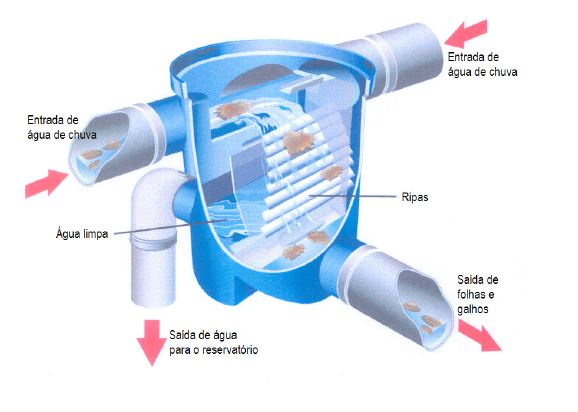
\includegraphics[scale=0.6]{captacao/10.png}
	 \caption{Sistema de filtro utilizado.}
	  \small{Fonte: \cite{ECOCASA}}
\end{figure}

A tabela 6 apresenta o tipo da água da chuva, com o filtro usado e a desinfecção requerida, no parque será utilizada água não potável, pois apresenta filtros e tratamento químico com cloro, para no caso de contato com a pele, não cause nenhum efeito colateral.

\begin{table}[h]
\centering
\caption{tipo da agua e propriedades exigidas.}
\label{tipo da agua e propriedades exigidas}
\begin{tabular}{llll}
 &  &  &  \\ \hline
\multicolumn{1}{|l|}{} & \multicolumn{3}{l|}{Aplicações Básicas} \\ \hline
\multicolumn{1}{|l|}{Tratamento necessário} & \multicolumn{1}{l|}{Potável} & \multicolumn{1}{l|}{Não potável} & \multicolumn{1}{l|}{Rega e Limpeza} \\ \hline
\multicolumn{1}{|l|}{\begin{tabular}[c]{@{}l@{}}Filtros a serem\\  instalados\end{tabular}} & \multicolumn{1}{l|}{\begin{tabular}[c]{@{}l@{}}Filtro para sedimentos e no \\ mínimo outro de carvão \\ ativado, para eliminar \\ produtos químicos.\end{tabular}} & \multicolumn{1}{l|}{\begin{tabular}[c]{@{}l@{}}Filtro de sedimentos e \\ partículas alem de \\ tratamento com cloro.\end{tabular}} & \multicolumn{1}{l|}{\begin{tabular}[c]{@{}l@{}}É suficiente um filtro por \\ gravidade de pedras.\end{tabular}} \\ \hline
\multicolumn{1}{|l|}{Desinfecção requerida} & \multicolumn{1}{l|}{Necessário/fundamental} & \multicolumn{1}{l|}{Necessário} & \multicolumn{1}{l|}{Não é necessária} \\ \hline
\end{tabular}
\end{table}

A qualidade da água é definida pela sua composição física, química e bacteriológica. Como a água da chuva captada não será direcionada para o consumo ela não precisa ser potável, portanto o tratamento necessário para ela é um cuidado com bactérias capazes de criar enfermidades ou qualquer organismo capazes de provocar enfermidades. \cite{sorgato2014analise}  Mesmo a água não sendo utilizada para o consumo ela deve ser corretamente tratada por entrar em contato com os seres humanos na irrigação, nas descargas do banheiro ou na limpeza, não podendo, então, conter bactérias causadoras de enfermidades.

A desinfecção de água de chuva poderá ser realizada através de sistema simples, como através de adição de cloro, para não inviabilizar economicamente o sistema. O cloro deverá ser aplicado de forma mais homogênea possível, devendo repetir a operação sempre que o teor de cloro ficar muito baixo alem de não alterar no pH da água. A desinfecção é um tratamento prioritário porque se uma água não for bem tratada e podendo estar contaminada poderá trazer sérios riscos à saúde. O preço do cloro é relativamente baixo, de em torno de 150 reais o pote de 10 kg.

Para bombeamento da água será utilizado uma bomba d’água acoplada a rede elétrica monofásica submersa de Ÿ de polegada que utiliza 300 watts e 220v ECCO - Anauger por ter um preço baixo, de aproximadamente 200 reais no mercado, com excelente vazão com pressão que alcança bombeamento de altura máxima de 50 metros.

O sistema de captação de água reduzirá notavelmente o consumo total de água do parque, e nos períodos de seca, essa água armazenada poderá ser devidamente utilizada para irrigação dos jardins próximos à área do banheiro, além de servir para o uso em descargas e limpeza dos pisos. O reuso da água da chuva que será instalado é um ótimo caminho para tornar o parque em um parque modelo de sustentabilidade.

Dessa forma, o custo de construção girará em torno de 4300 reais por local de instalação, contando com a mão-de-obra e com os materiais, e para a manutenção foi estipulado um valor de 200 reais por mês para mão de obra e purificação da água, assim em aproximadamente um ano a água economizada com a instalação desse sistema de captação cobrirá os custos iniciais, levando em consideração a quantidade de pessoas que frequentarão o parque e a quantidade de chuvas que pode variar a cada ano.

\section{Quanto custa o $M^{3}$ da CAESB?}

O parque mensalmente irá consumir:
\begin{itemize}
	\item 60.000L de água em descargas (60 $m^{2}$);
\end{itemize}

	
	Tendo em vista que durante 3 meses o abastecimento será feito pela companhia de abastecimento do DF. Calculando quanto o parque teria que pagar a CAESB em tributos mensalmente, utilizando as tarifas atualmente vigentes na companhia obtêm-se: 
	
\begin{table}[h]
\centering
\caption{Valor pago mensalmente a CAESB (estimativa)}
\label{Valor pago mensalmente a CAESB (estimativa)}
\begin{tabular}{lllll}
 &  &  &  &  \\ \hline
\multicolumn{1}{|l|}{Uso} & \multicolumn{1}{l|}{Consumo Mensal em L} & \multicolumn{1}{l|}{M3} & \multicolumn{1}{l|}{Tarifa} & \multicolumn{1}{l|}{Custo em Reais} \\ \hline
\multicolumn{1}{|l|}{Descargas} & \multicolumn{1}{l|}{60.000} & \multicolumn{1}{l|}{60} & \multicolumn{1}{l|}{10,82 (\textgreater10 $m{3}$)} & \multicolumn{1}{l|}{649,2} \\ \hline
\multicolumn{1}{|l|}{TOTAL} & \multicolumn{1}{l|}{} & \multicolumn{1}{l|}{} & \multicolumn{1}{l|}{} & \multicolumn{1}{l|}{649,20 BRL} \\ \hline
\end{tabular}
\end{table}

Mensalmente a administração do Parque Urbano e Vivencial do Gama gastaria R\$ 649,20 reais em conta de água e nos outros 3 meses onde será utilizada água pública R\$ 1.947,60 reais. Caso o parque fosse pagar pelos seus 720m3 utilizados anualmente essa conta seria de R\$ 7.790,40 que deveriam ser pagos a CAESB. Entretanto, como o parque gasta apenas R\$ 1.947,60 em tributos à CAESB, a economia acaba sendo de R\$ 5.842,80 anualmente em conta de água. 

\chapter{Postes}

\section{Adapta\c{c}\~ao do poste PTS para sistema ON-GRID}

	A Resolu\c{c}\~ao Normativa 482 da ANEEL- estabeleceu as condi\c{c}\~oes gerais para a conex\~ao \`a rede da microgera\c{c}\~ao (pot\^encia instalada menor que 100kWp) e minigera\c{c}\~ao (pot\^encia instalada entre 100kWp e 1MWp) distribu\'ida no Brasil e criou o Sistema de Compensa\c{c}\~ao de Energia. Tal sistema permite que sistemas fotovoltaicos  e outras formas de gera\c{c}\~ao de energia a partir de fontes renov\'aveis com at\'e 1MW de pot\^encia  instalados em resid\^encias e empresas  se conectem a rede el\'etrica de forma simplificada, atendendo o consumo local e in/jetando o excedente na rede, gerando cr\'editos de energia\cite{SMARTLY}. 
	Desta forma, \'e poss\'ivel praticamente zerar a conta de luz com o uso da energia solar, pagando apenas o custo de disponibilidade da rede. Quando um sistema fotovoltaico estiver gerando eletricidade, esta ser\'a consumida no local. Caso a gera\c{c}\~ao seja maior que o consumo, o excedente \'e injetado na rede el\'etrica, gerando cr\'editos de energia. Quando a gera\c{c}\~ao for menor do que o consumo, ser\'a utilizada a energia da pr\'opria rede el\'etrica. Os cr\'editos de energia possuem o mesmo valor da eletricidade da rede e podem ser utilizados para abater o consumo, diminuindo assim o valor da conta de energia, e possuem validade de at\'e 36 meses para serem resgatados.
	Os sistemas \textit{ON-GRID} ou \textit{GRID-TIE}, existentes atualmente s\~ao compostos de um inversor, capaz de converter a corrente cont\'inua, produzida pelos pain\'eis, em corrente alternada em sincronia com a rede el\'etrica.
	O Inversor \textit{grid tie} Central, \'e o ideal para a aplica\c{c}\~ao na \'area de conviv\^encia social do parque, pois um \'unico inversor desse tipo \'e capaz de atender toda a demanda dos postes solares do Parque. Ele recebe energia de v\'arios pain\'eis solares, ligados em s\'erie e paralelo, estabilizando com um \'unico otimizador MPPT e fazendo sua fun\c{c}\~ao de inversor DC/AC. H\'a um ganho de custo por utilizar menor n\'umero de inversores. Ele seria uma central que receberia a energia excedente produzida pelos postes PTS 410 e injetaria na rede el\'etrica, caso a energia produzida no poste n\~ao seja suficiente para a manuten\c{c}\~ao do mesmo, ele permite que energia da rede seja utilizada nos postes. Os inversores centrais s\~ao comumente utilizados em sistemas fotovoltaicos com pot\^encias entre 20 e 400 kW, figura abaixo \cite{SUNLABPTS}.
	
\begin{figure}[H]
	\centering
	\label{InversorCentral}
		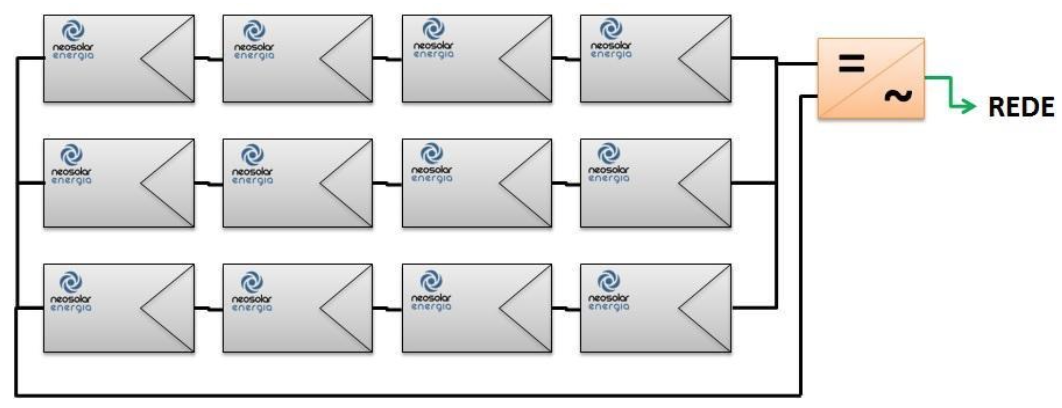
\includegraphics[keepaspectratio=true,scale=0.9]{figuras/InversorCentral.png}
	\caption{Inversor Central}
	\small{Fonte: \cite{NEOSOLAR} }
\end{figure}
	
	Na \'area de conviv\^encia social um \'unico inversor central ir\'a receber toda a pot\^encia produzida pelos pain\'eis solares dos  13 postes. Sabendo que cada poste produz uma pot\^encia de 250 W, o inversor central ir\'a receber em m\'edia 3250 W, ou seja, sua gera\c{c}\~ao com irradia\c{c}\~ao m\'axima. Portanto optou-se por um inversor Fronius IG Plus 5V-1 (03.503.012), da neosolar energia, que recebe uma pot\^encia de at\'e 4000W custa em m\'edia R\$ 8.400,00.
	Para a Pista de Cooper devido sua extens\~ao, \'e necess\'ario outro tipo de inversor, pois um inversor central n\~ao conseguiria receber toda energia produzida nos postes, que ficam em uma \'area muito grande do Parque. Cada inversor recebe uma s\'erie ou string e v\'arios inversores s\~ao utilizados em paralelo, cada um com seu otimizador MPPT \cite{SUNLABPTS}. Essa configura\c{c}\~ao permite maior flexibilidade, como diferentes orienta\c{c}\~oes para cada string.  O Inversor grid tie modular \'e um sistema fotovoltaico modularizado, com um otimizador para cada s\'erie (string), por\'em h\'a um ganho de custo com a utiliza\c{c}\~ao de um \'unico inversor, quando comparamos com os inversores modulares. A maioria dos inversores atualmente utilizados s\~ao modulares,  proporcionando flexibilidade e ganhos de custo, tornando poss\'ivel fragmentar os postes da pista de Cooper em strings(conjuntos) que utilizam o mesmo inversor, que s\~ao ligados a rede, figura a seguir.
	
\begin{figure}[H]
	\centering
	\label{InversorModular}
		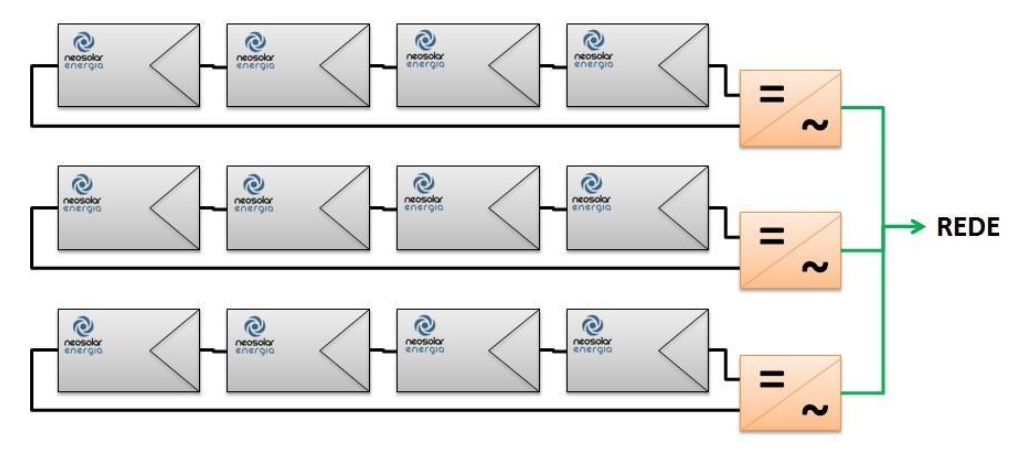
\includegraphics[keepaspectratio=true,scale=0.9]{figuras/InversorModular.png}
	\caption{Inversor Modular}
	\small{Fonte: \cite{NEOSOLAR} }
\end{figure}
	
	A pista de Cooper cont\'em 103 postes, e deve ser dividida em 4 strings. Cada string, deve se conter 26 postes, e um inversor que receba energia gerada por eles e injete na rede, ele dever\'a se localizar em um ponto intermedi\'ario de cada string. Sabendo que cada poste PTS 315 gera uma pot\^encia de 140 W, cada string ir\'a produzir 3640 W de pot\^encia, e por seguran\c{c}a de projeto optou-se por um inversor com pot\^encia de entrada (pot\^encia produzida na string) 4.260W, da linha de inversores produzida pela  Fronius ( Fronius IG Plus 5V-1 (03.503.012)), da neosolar energia. Cada inversor custa em m\'edia R\$ 8.400,00, e \'e o mesmo utilizado na \'area de conviv\^encia social mudando apenas o arranjo do sistema de inversor central para inversor modular \cite{SUNLABPTS}. 
	
	Especifica\c{c}\~oes t\'ecnicas do fabricante
	
\begin{itemize}
         \item Entrada
                  \begin{itemize}
                            \item Pot\^encia m\'axima de entrada: 4260W
                            \item Voltagem m\'axima de entrada: 600Vcc
                            \item Faixa de Voltagem do MPP: (230Vcc a 500Vcc)
                            \item Voltagem m\'inima de entrada: 230Vcc
                            \item Voltagem para inicializa\c{c}\~ao: 260Vcc
                            \item Corrente m\'axima de entrada: 18,6A
                  \end{itemize}
         \item Saida
                  \begin{itemize}
                            \item Pot\^encia nominal de sa\'ida: 4000W
                            \item Voltagem de sa\'ida (faixa): 180Vca a 270Vca
                            \item Frequ\^encia de sa\'ida: 60Hz
                            \item Corrente m\'axima de sa\'ida: 17,4A
                  \end{itemize}
          \item Outras caracter\'isticas 
                  \begin{itemize}
                            \item Efici\^encia M\'axima: 95,7\%
                            \item Consumo interno (noite): <1W
                            \item Temperatura de Opera\c{c}\~ao: -25$^{o}$C a +50$^{o}$C
                            \item Frequ\^encia de sa\'ida: 60Hz
                            \item Especifica\c{c}\~oes Mec\^anicas
                                    \begin{itemize}
                                             \item Dimens\~oes (L x A x P)mm: (673 x 434 x 250)
                                             \item Peso: 23,8Kg
                                    \end{itemize}
                  \end{itemize}
\end{itemize}

\section{Medidor bidirecional}

	Para o sistema de compensa\c{c}\~ao protocolada pela ANEEL, a energia produzida em uma regi\~ao de microgera\c{c}\~ao, antes de ser injetada na rede deve passar em um medidor bidirecional, no qual mede a energia produzida ( que \'e injetada na rede), e a energia que \'e utilizada da rede nos momentos de baixa gera\c{c}\~ao (\`a noite). Observe a figura abaixo, de um modelo de sistema residencial.
	
\begin{figure}[H]
	\centering
	\label{ModeloResidencial}
		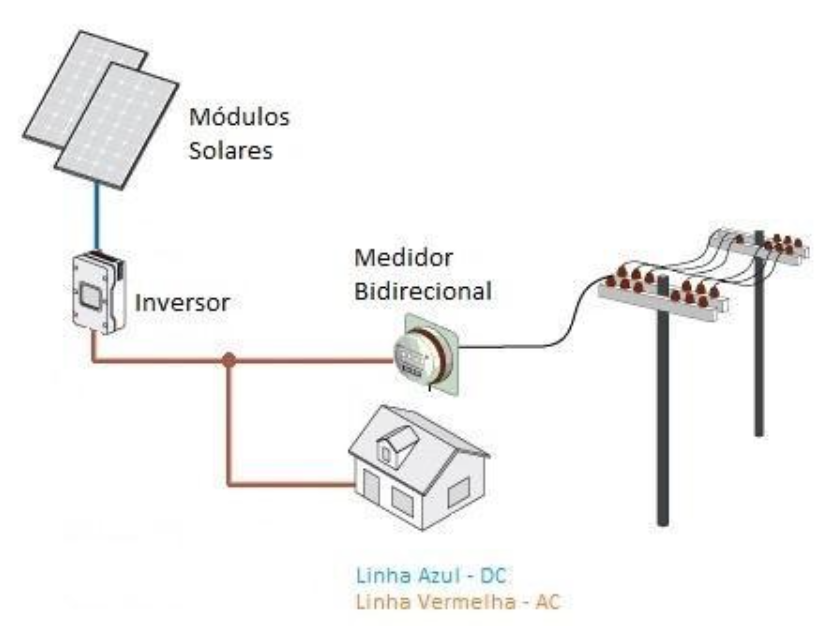
\includegraphics[keepaspectratio=true,scale=0.9]{figuras/ModeloResidencial.png}
	\caption{Modelo Residencial}
	\small{Fonte: \cite{SMARTLY} }
\end{figure}
	
	Os medidores bidirecionais existentes no mercado atualmente, que atuam em uma voltagem de 220V, no caso do Parque custam em m\'edia R\$ 360,00 cada. Os medidores s\~ao fornecidos pela Noesolar, e s\~ao necess\'arios  um medidor para cada inversor. Sabendo que s\~ao neces\'arios cinco inversores, consequentemente ser\~ao usados cinco medidores. Assim temos que o custo total dos medidores \'e de :
	
	\textbf{Custo total dos medidores: 5 unidades x 360 pre\c{c}o unit\'ario = R\$ 1800,00. }
	
\section{Cabeamento e Conectores}

	S\~ao espec\'ificos para sistemas fotovoltaicos e usados para as conex\~oes entre pain\'eis e inversores (lado corrente cont\'inua - CC) e tamb\'em entre inversores e rede el\'etrica (lado corrente alternada - AC). Devem ser resistentes \`a radia\c{c}\~ao ultravioleta e a intemp\'eries, al\'em de suportar temperaturas elevadas, t\'ipicas nesse sistema. Os cabos t\^em se\c{c}\~ao de 4 m$m^{2}$ ou 6 m$m^{2}$ e os conectores seguem o padr\~ao conhecido como MC4 \cite{NEOSOLAR}.
	Os conectores tipo MC4 s\~ao utilizados especificamente em  sistemas fotovoltaicos . Este tipo de conector melhora a qualidade da instala\c{c}\~ao, facilita a conex\~ao entre pain\'eis e apresentam melhor durabilidade quando expostos as condi\c{c}\~oes clim\'aticas t\'ipicas de sistemas fotovoltaicos por grandes per\'iodos, como insola\c{c}\~ao e umidade, figura a seguir.
	
\begin{figure}[H]
	\centering
	\label{ConectoresMC4}
		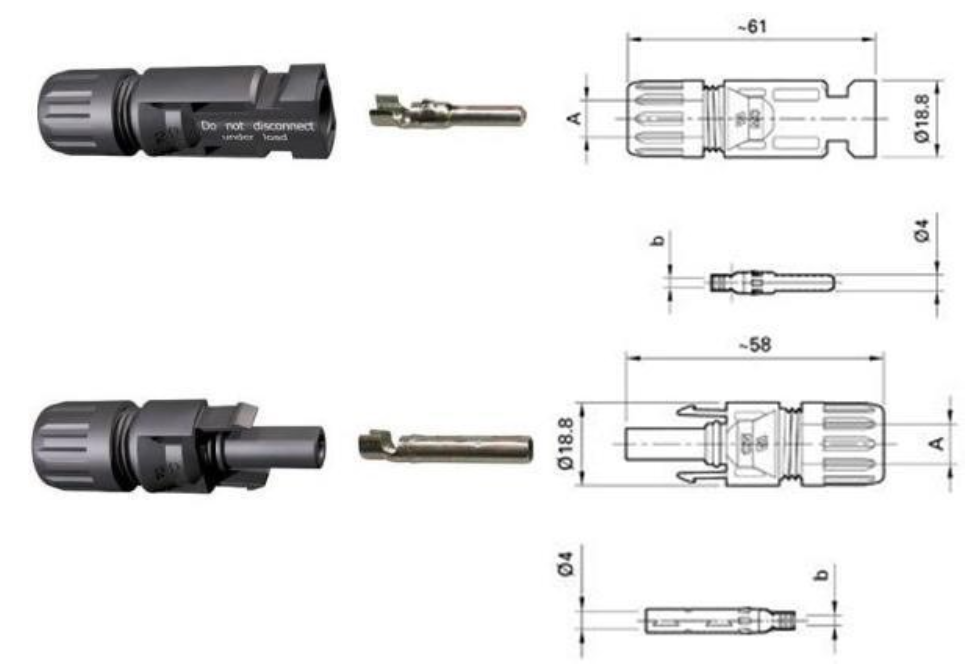
\includegraphics[keepaspectratio=true,scale=0.9]{figuras/ConectoresMC4.png}
	\caption{Conectores MC4}
	\small{Fonte: \cite{NEOSOLAR} }
\end{figure}
	
	Cada par de conectors macho/ f\^emea necess\'arios em cada placa, custam  em m\'edia R\$ 14,00 de acordo com o fabricante Sunlab, sabendo que s\~ao 103 placas utilizadas na pista de cooper e 13 na \'area de conviv\^encia social, totalizando 116 placas, pode-se concluir que o custo total dos conectores \'e de :
	
	\textbf{Custo total dos conectores = 116 unidades x 14 pre\c{c}o unit\'ario = R\$ 1.640,00.}
	
	Aos conectores das placas s\~ao acoplados cabos que devem chegar at\'e os inversores e posteriormente \`a rede, os fios conectores indicados pela empresa Sunlab,( que faz parte de um grupo de empresas voltadas para a energia fotovolt\'aica), s\~ao :
	
Par de condutores flex\'iveis Conduspar com espessura de 6,0m$m^{2}$ de alta qualidade com certifica\c{c}\~ao INMETRO. Os cabos s\~ao feitos em cobre eletrol\'itico com isolamento para tens\~oes nominais at\'e 450/7.\cite{NEOSOLARCASASOLAR}
O Par \'e constitu\'ido de um metro de  fio preto e um metro de fio vermelho, de di\^ametro de 6mm, e custa R\$ 4, 56. Sabendo que eles s\~ao utilizados para fazer a liga\c{c}\~ao em paralelo entre os postes, que est\~ao ligados uns ao outros em strings. Portanto sabendo que o per\'imetro da pista de Cooper em ciclo completo em volta da pista \'e de 6684,58 m o per\'imetro da \'area de conviv\^encia social, 400 m poss\'ivel determinar o custo aproximado dos cabos utilizados, para fazer a conex\~ao dos postes na rede. O per\'imetro total da \'area de aplica\c{c}\~ao dos postes \'e de 7044,58 metros, assim o custo \'e de:

	\textbf{Custo aproximado do cabeamento: Pre\c{c}o unit\'ario por metro R\$ 4,56 x Per\'imetro total  7.044,58 m  =  R\$ 32.123,30.}
	
	Assim o valor aproximado para o cabeamento que liga os postes para aos inversores \'e de R\$ 32.123,30. Esse valor \'e vari\'avel em fun\c{c}\~ao da organiza\c{c}\~ao e localiza\c{c}\~ao dos inversores das strings, al\'em da dist\^ancia da rede P\'ublica ao local de instala\c{c}\~ao dos inversores. A rede atualmente n\~ao passa nas imedia\c{c}\~oes do Parque, mas o projeto em andamento indica que essa rede ser\'a instalada com certa proximidade, facilitando a liga\c{c}\~ao dos inversores com a rede \'e diminuindo uma poss\'ivel oscila\c{c}\~ao do custo total dos cabos.
	
\section{Custo total da ilumina\c{c}\~ao}

	Foram levantados os custos do projeto de ilumina\c{c}\~ao de acordo com os valores informados por um revendedor (infinittosolar) da fabricante dos postes (sunlab).
	Para o modelo PTS 315, que ser\'a usado em toda a pista de cooper, temos  o pre\c{c}o unit\'ario do  kit de R\$ 5.172,06, que inclui lumin\'aria, bra\c{c}o da lumin\'aria, caixa com controlador, painel e suporte para pain\'eis regul\'avel, mais um custo adicional de R\$ 1.152,00 do poste. Para o modelo PTS 410, que ser\'a usados em estacionamentos e \'areas de conv\'ivio social, temos o pre\c{c}o unit\'ario do kit de R\$ R\$ 8.080,00 que inclui lumin\'aria, bra\c{c}o da lumin\'aria, caixa com controlador, painel e suporte para pain\'eis regul\'avel, mais um custo adicional de R\$ 1.357,00 do poste. A revendedora tamb\'em cobra uma taxa para instala\c{c}\~ao dos postes, que equivale a R\$253,00 cada poste.
	Apesar da ado\c{c}\~ao de dois sistemas de invers\~ao (Central e Modular) de corrente cont\'inua para corrente alternada. Os 4 inversores utilizados para a pista de Cooper, s\~ao do mesmo modelo utilizada nas \'areas de conviv\^encia social r( Fronius IG Plus 5V-1 (03.503.012)). No total s\~ao utilizados 5 inversores, e cada uma custa em m\'edia R\$ 8.400,00, totalizando um custo de implementa\c{c}\~ao do equipamento no Poste em cerca de R\$ 42.000,00.
	No projeto ser\~ao utilizados 103 postes do modelo PTS 315, ent\~ao utilizando a f\'ormula Ct = (Ck + Cp + Ci) x Qp , onde Ct \'e o custo total, Ck \'e o custo do kit, Cp \'e o custo do poste, Ci \'e o custo de instala\c{c}\~ao, e Qp \'e quantidade de postes temos (5172+1152+253)x103 = R\$ 677.431,00 e 13 postes do modelo PTS 410 , onde, utilizando a mesma f\'ormula, temos (8080+1357+253)x13 = R\$ 125.970,00 .Logo, somando o custo total dos dois modelos de poste, mais o custo de implementa\c{c}\~ao dos inversores, dos medidores, dos conectores e do cabeamento temos um custo total para ilumina\c{c}\~ao de 677.431 + 125.970 + 42.000 + 1.800 + 1640 + 32.123,30 = R\$ 880.964,30.
	Com a utiliza\c{c}\~ao dos inversores, n\~ao se faz mais necess\'ario a utiliza\c{c}\~ao de baterias em cada poste. Cada bateria spiracell (bateria \textit{"YELLOW"}, cujo c\'odigo \'e 93528,e o modelo \'e  D31A) da Sunlab para os postes PTS custa R\$ 1.352,94 cada. Como no total s\~ao 116 postes contando \'area de conviv\^encia e pista de Cooper, temos uma economia de 116x1352,94 = R\$ 156.941,04 .	
	Apesar da necessidade de manuten\c{c}\~ao dos inversores e do pagamento da taxa de ilumina\c{c}\~ao a empresa concession\'aria de energia, a utiliza\c{c}\~ao de um sistema \textit{ON-GRID}, o qual torna desnecess\'ario o uso de baterias torna o Projeto bem mais barato. A vida \'util de cada Inversor \'e de aproximadamente de 10 a 15 anos, e se aproxima da vida \'util das baterias, ou seja, os gastos anteriores que seriam necess\'arios com a manuten\c{c}\~ao das mesmas, agora ser\~ao utilizados com a manuten\c{c}\~ao dos inversores, tornando equivalente tais despesas. Com isso a aplica\c{c}\~ao desse sistema \'e mais barata que a utiliza\c{c}\~ao de baterias para a alimenta\c{c}\~ao dos postes.
	
\section{Balan\c{c}o energ\'etico dos postes}

	Produ\c{c}\~ao e consumo dos postes
	
	Sabendo que ser\~ao utilizados 103 Postes na pista de Cooper no modelo Sunlab PTS-315, o qual possui uma placa solar com pot\^encia 140W, e 13 postes  Sunlab PTS-410, o qual possui uma placa solar com pot\^encia 250 W, pode-se estimar a produ\c{c}\~ao mensal dos postes em energia. Nas figuras 1 e 2 abaixo, de acordo com o fabricante (Sunlab), pode-se obter , a produ\c{c}\~ao m\'edia mensal de cada placa, e consequentemente a produ\c{c}\~ao mensal de todos os postes existentes no Parque.
	
\begin{figure}[H]
	\centering
	\label{PlacaPistadeCooper}
		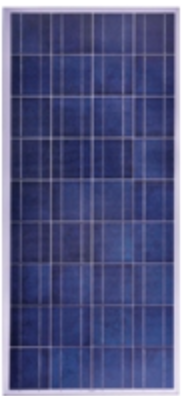
\includegraphics[keepaspectratio=true,scale=0.9]{figuras/PlacaPistadeCooper.png}
	\caption{Placa usada na Pista de Cooper}
	\small{Fonte: \cite{NEOSOLARCASASOLAR} }
\end{figure}

\begin{figure}[H]
	\centering
	\label{PlacaConvivenciaSocial}
		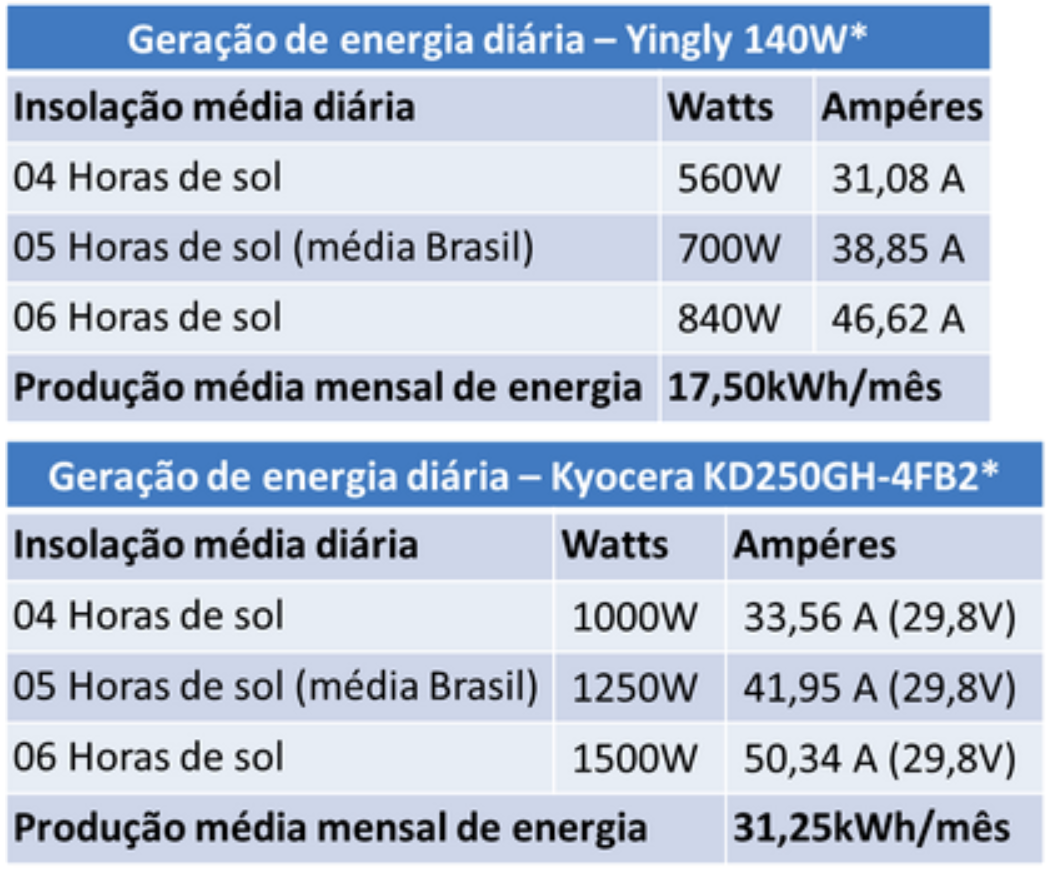
\includegraphics[keepaspectratio=true,scale=0.9]{figuras/PlacaConvivenciaSocial.png}
	\caption{Placa usada na  \'area de conviv\^encia social}
	\small{Fonte: \cite{NEOSOLARCASASOLAR} }
\end{figure}
	
	Com a produ\c{c}\~ao mensal de cada placa, \'e poss\'ivel determinar a produ\c{c}\~ao mensal de todos os Postes:
Multiplicando a produ\c{c}\~ao mensal, da placa usada na pista de Cooper pelo numero de postes temos:
103x17,5=1802,5 KWh mensal

Multiplicando a produ\c{c}\~ao mensal, da placa usada na \'area de conviv\^encia social pelo numero de postes temos:
13x31,25=406,25 KWh mensal

\begin{table}[H]
\caption{Caracter\'isticas dos Componentes dos Postes} 
\label{ComponentesDosPostes}
\begin{center}
\begin{tabular}{|p{1cm}lp{1cm}lp{1cm}lp{1cm}lp{1cm}lp{1cm}lp{1cm}l} \hline

MODELO DO POSTE &TIPO DE LUMIN\'ARIA &CONSUMO DA LUMIN\'ARIA(W) &N$^{o}$ DE LUMIN\'ARIAS &TIPO DE CONTROLADOR &CONSUMO DO CONTROLADOR(W) &N$^{o}$ DE CONTROLADORES\\ \hline 

PTS-315         & ILC               & 48                      & 1                & LZP-10              & 0,0408                    & 1                   \\ \hline
PTS-410         & ILC               & 48                      & 2                & LZP-20              & 0,0408                    & \\ \hline  

 \end{tabular}
\end{center}
\end{table}

	Assim pode-se obter o consumo para cada modelo de Poste, de acordo com as especifica\c{c}\~oes  da tabela \ref{ComponentesDosPostes}:
	
\begin{enumerate}
         \item Consumo do poste PTS-315:
                  \begin{itemize}
                            \item Lumin\'aria : 48 x 12h x 30dias = 17280 Wh mensal
                            \item Controlador LZP-10: 0,0408 x 24h x 30dias = 29,376 Wh mensal 
                            \item Consumo Total por poste :17309,376 Wh mensal
                            \item Consumo total pelo modelo: 17309,376 x 103 = 1782,86 KWh mensal
                  \end{itemize}
         \item Consumo do poste PTS- 410:
                  \begin{itemize}
                            \item Lumin\'aria (2 lumin\'arias): 2 x 48 x 12h x 30 dias = 34560 Wh mensal
                            \item Controlador LZP-20:  0,0408 x 24h x 30 dias = 29,376 Wh mensal  
                            \item Consumo total por poste: 34589,376 Wh mensal
                            \item Consumo total pelo modelo:  34589,376 x 13 = 449,662 KWh mensal
                  \end{itemize}
\end{enumerate}

	Assim tem-se que o consumo mensal total de ambos os postes, somando os valores encontrados acima \'e de  \'e cerca de 2232,52 KWh mensal.
	
\chapter{Especifações do Sistema Solar Proposto}

O Sistema será composto de sete inversores, sendo um de 6000W para a sede administrativa, um de 3000W para cada um dos quiosques e um de 1500W para cada um dos banheiros e guaritas. Os modelos recomendados são: Inversor Fronius IG Plus 60 V-1 (6KW), Inversor Fronius Galvo 3.0-1 (3KW) e Inversor Fronius Galvo 1.5-1 (1,5KW).
	Alem dos inversores, serão utilizados painéis fotovoltáicos de silicio policristalino, sendo vinte e dois de para a sede administrativa, três para cada um dos banheiros e três para cada uma das guaritas, todos retangulares e de 250 W. No caso do quiosque, devido ao formato do telhado ser diferenciado, é necessário utilizar algumas placas triangulares, ficando com 6 placas retangulares de 1,2x1,3m(240W) e 12 placas triangulares de 1,2x1,2m(140W). Abaixo temos os modelos e especificações das placas utilizadas para o cálculo.
	Especificações do Painel Solar Fotovoltaico Policristalino de 250W da Kyocera Solar (retangular).
	
\begin{figure}[H]
	\centering
	\label{Painel Solar Fotovoltaico Policristalino de 250W da Kyocera Solar}
		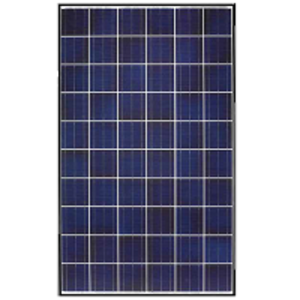
\includegraphics[keepaspectratio=true,scale=0.9]{solar/1.png}
	\caption{Painel Solar Fotovoltaico Policristalino de 250W da Kyocera Solar}
	\small{Fonte: \cite{KYOCERA}}
\end{figure}

\begin{itemize}
	\item Potência máxima (Pmax): 250Wp;
	\item Tolerância: +5\%/-3\%;
	\item Tensão em circuito aberto (Voc): 36,9V;
	\item Tensão de Pico (Vmpp): 29,8V;
	\item Corrente de curto-circuito (Isc): 9,09A;
	\item Corrente de Pico (Impp): 8,39A;
	\item Voltagem máxima do sistema: 1000V; 
	\item Tipo de célula: Silício Policristalino;
	\item Dimensões painel: 1662 x 990 x 46 (mm);
	\item Peso: 20 kg; 
\end{itemize}

Especificações do Painel Solar Fotovoltáico Policristalino de 120W da Coenergia Group (triangular)

\begin{figure}[H]
	\centering
	\label{Painel Solar Fotovoltáico Policristalino de 120W da Coenergia Group (Triangular)}
		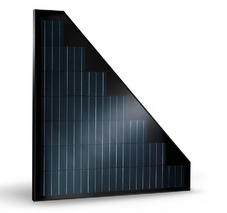
\includegraphics[keepaspectratio=true,scale=0.9]{solar/2.png}
	\caption{Painel Solar Fotovoltáico Policristalino de 120W da Coenergia Group (Triangular)}
	\small{Fonte: \cite{KYOCERA}}
\end{figure}

\begin{itemize}
	\item Potência máxima (Pmax): 120Wp;
	\item Tolerância: +3\%/0\%;
	\item Tensão em circuito aberto (Voc): 17,69V;
	\item Tensão de Pico (Vmpp): 14,75V;
	\item Corrente de curto-circuito (Isc): 9,26A;
	\item Corrente de Pico (Impp): 8,14A;
	\item Voltagem máxima do sistema: 1000V;
	\item Tipo de célula: Silício Policristalino;
	\item Dimensões painel: 1200 x 1200 x 40 (mm);
	\item Peso: 11 kg;
\end{itemize}

Especificações do painel Solar Fotovoltáico Policristalino de 240W da Coenergia Group (retangular)

\begin{figure}[H]
	\centering
	\label{Painel Solar Fotovoltáico Policristalino de 240W da Coenergia Group (Retangular)}
		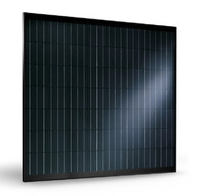
\includegraphics[keepaspectratio=true,scale=0.9]{solar/3.png}
	\caption{Painel Solar Fotovoltáico Policristalino de 240W da Coenergia Group (Retangular)}
	\small{Fonte: \cite{COENERGIA}}
\end{figure}

\begin{itemize}
	\item Potência máxima (Pmax): 240Wp;
	\item Tolerância: +3\%/0\%;
	\item Tensão em circuito aberto (Voc): 35,38V;
	\item Tensão de Pico (Vmpp): 29,5V;
	\item Corrente de curto-circuito (Isc): 9,26A;
	\item Corrente de Pico (Impp): 8,14A;
	\item Voltagem máxima do sistema: 1000V;
	\item Tipo de célula: Silício Policristalino;	
	\item Dimensões painel: 1200 x 1300 x 40 (mm);
	\item Peso: 18 kg;
\end{itemize}

\section{Tempo de retorno para a placa solar}

Feito para ser durável, o Sistema gerador solar \textit{on-grid} só precisa ser trocado a cada 25 anos. Esse é o tempo em que os painéis levam para ter sua eficiência reduzida para até 80\%, sendo recomendada a troca. Os inversores podem ter sua garantia estendida para até 20 anos, podendo funcionar pelos 25 anos do sistema.

Através das estimativas realizadas, obteve-se que para os edifícios a serem construídos no parque, o consumo elétrico médio mensal será de 2055 Kwh. Dados obtidos no site da CEB (Companhia Energética de Brasília) mostram que, para o parque do Gama (Classificado como poder público) o preço atual do Kwh é de R\$ 0,46761. Sendo assim, o gasto mensal com energia, seria de R\$ 960,94 e o anual R\$ 11.531,28, de forma que o investimento no sistema solar teria seu retorno¹ em aproximadamente 12 anos e 7 meses e a quantia economizada ao final de 25 anos seria R\$ 143.103,18¹.

Porém, como podemos ver no gráfico abaixo, ao analisar os dados dos últimos 12 meses, nota-se a tendência do valor do Kwh crescer, o que pode antecipar o tempo de retorno e aumentar a quantia economizada. 

\begin{figure}[H]
	\centering
	\label{Gráfico representando custo por Kwh de energia elétrica.}
		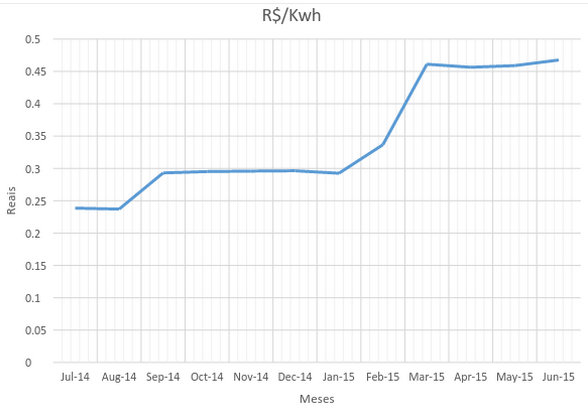
\includegraphics[keepaspectratio=true,scale=0.9]{solar/4.png}
	\caption{Gráfico representando custo por Kwh de energia elétrica.}
	\small{Imagem de autoria própria}
\end{figure}

\chapter{Custos}

\section{Balanço económico cercamento}

 Foram levantados os custos do cercamento, que estão detalhados na tabela x, de acordo com os dados fornecidos pelo SINAPI (Sistema Nacional de Preços e Índices para Construção Civil), que é um órgão criado pela Caixa EconÎmica Federal (CEF) que tem por objetivo efetuar o orçamento analítico e a análise orçamentária de projeto-tipo e projetos específicos e efetuar o acompanhamento de preços, de custos e de índices da construção civil na área de fomento (habitação, saneamento e infra-estrutura urbana). 
 
Apresenta-se também, para melhor esclarecimento dos custos, na seguinte tabela, o BDI (Bonificação de Despesas Indiretas) que é o elemento orçamentário destinado a cobrir todas as despesas que, num empreendimento (obra ou serviço), segundo critérios claramente definidos. Classificam-se como indiretas (por simplicidade, as que não expressam diretamente nem o custeio do material nem o dos elementos operativos sobre o material, mão-de-obra, equipamento-obra, instrumento-obra etc.) e, também, necessariamente, atender o lucro.

O BDI da tabela foi estimado a partir da Média de composições compilados no Sistema Nacional de Pesquisa de Custos e Indices (SINAPI) a partir de serviços similares.



\begin{landscape}
\begin{table}[h]
\centering
\caption{Custos devido ao cercamento completo.}
\label{Custos devido ao cercamento completo.}
\begin{tabular}{lllllllll}
 &  &  &  &  &  &  &  &  \\ \hline
\multicolumn{1}{|l|}{ITEM} & \multicolumn{1}{l|}{DESCRIÇÃO} & \multicolumn{1}{l|}{UNID} & \multicolumn{1}{l|}{QTD} & \multicolumn{2}{l|}{MATERIAL} & \multicolumn{2}{l|}{MÃO-DE-OBRA} & \multicolumn{1}{l|}{TOTAL} \\ \hline
\multicolumn{1}{|l|}{} & \multicolumn{1}{l|}{} & \multicolumn{1}{l|}{} & \multicolumn{1}{l|}{} & \multicolumn{1}{l|}{UNIT} & \multicolumn{1}{l|}{TOTAL} & \multicolumn{1}{l|}{UNIT} & \multicolumn{1}{l|}{TOTAL} & \multicolumn{1}{l|}{} \\ \hline
\multicolumn{1}{|l|}{1.0} & \multicolumn{1}{l|}{SERVIÇOS PRELIMINARES} & \multicolumn{1}{l|}{} & \multicolumn{1}{l|}{} & \multicolumn{1}{l|}{} & \multicolumn{1}{l|}{419,51} & \multicolumn{1}{l|}{} & \multicolumn{1}{l|}{R\$25,61} & \multicolumn{1}{l|}{R\$445,12} \\ \hline
\multicolumn{1}{|l|}{01/01/2015} & \multicolumn{1}{l|}{Taxa da ART} & \multicolumn{1}{l|}{ud} & \multicolumn{1}{l|}{1} & \multicolumn{1}{l|}{R\$158,08} & \multicolumn{1}{l|}{R\$158,08} & \multicolumn{1}{l|}{} & \multicolumn{1}{l|}{R\$ -} & \multicolumn{1}{l|}{R\$158,08} \\ \hline
\multicolumn{1}{|l|}{01/02/2015} & \multicolumn{1}{l|}{\begin{tabular}[c]{@{}l@{}}Placa da obra em chapa\\ galvanizada\end{tabular}} & \multicolumn{1}{l|}{$m^{2}$} & \multicolumn{1}{l|}{1} & \multicolumn{1}{l|}{R\$261,43} & \multicolumn{1}{l|}{R\$261,43} & \multicolumn{1}{l|}{R\$25,61} & \multicolumn{1}{l|}{R\$25,61} & \multicolumn{1}{l|}{R\$287,04} \\ \hline
\multicolumn{1}{|l|}{2.0} & \multicolumn{1}{l|}{ADMINISTRAÇÃO LOCAL} & \multicolumn{1}{l|}{} & \multicolumn{1}{l|}{} & \multicolumn{1}{l|}{} & \multicolumn{1}{l|}{R\$600,00} & \multicolumn{1}{l|}{} & \multicolumn{1}{l|}{R\$3.817,00} & \multicolumn{1}{l|}{R\$4.417,00} \\ \hline
\multicolumn{1}{|l|}{02/01/2015} & \multicolumn{1}{l|}{\begin{tabular}[c]{@{}l@{}}Mobilização de pessoal \\ e equipamentos/ferramentas\end{tabular}} & \multicolumn{1}{l|}{ud} & \multicolumn{1}{l|}{1} & \multicolumn{1}{l|}{R\$400,00} & \multicolumn{1}{l|}{R\$400,00} & \multicolumn{1}{l|}{} & \multicolumn{1}{l|}{R\$ -} & \multicolumn{1}{l|}{R\$400,00} \\ \hline
\multicolumn{1}{|l|}{02/02/2015} & \multicolumn{1}{l|}{\begin{tabular}[c]{@{}l@{}}Desmobilização de pessoal\\  e equipamentos/ferramentas\end{tabular}} & \multicolumn{1}{l|}{ud} & \multicolumn{1}{l|}{1} & \multicolumn{1}{l|}{R\$200,00} & \multicolumn{1}{l|}{R\$200,00} & \multicolumn{1}{l|}{} & \multicolumn{1}{l|}{R\$ -} & \multicolumn{1}{l|}{R\$200,00} \\ \hline
\multicolumn{1}{|l|}{02/03/2015} & \multicolumn{1}{l|}{Encarregado} & \multicolumn{1}{l|}{mês} & \multicolumn{1}{l|}{1} & \multicolumn{1}{l|}{} & \multicolumn{1}{l|}{0} & \multicolumn{1}{l|}{3.817,00} & \multicolumn{1}{l|}{3.817,00} & \multicolumn{1}{l|}{R\$3.817,00} \\ \hline
\multicolumn{1}{|l|}{3.0} & \multicolumn{1}{l|}{GRADIL} & \multicolumn{1}{l|}{} & \multicolumn{1}{l|}{} & \multicolumn{1}{l|}{} & \multicolumn{1}{l|}{} & \multicolumn{1}{l|}{} & \multicolumn{1}{l|}{} & \multicolumn{1}{l|}{} \\ \hline
\multicolumn{1}{|l|}{03/01/2015} & \multicolumn{1}{l|}{\begin{tabular}[c]{@{}l@{}}Execução dos pilares\\ chumbados com \\ dimensões de 60x40x \\ 1,55mm,inclusive escavação,\\  remoção, botafora.\end{tabular}} & \multicolumn{1}{l|}{ud} & \multicolumn{1}{l|}{1671} & \multicolumn{1}{l|}{R\$6,94} & \multicolumn{1}{l|}{R\$11.596,74} & \multicolumn{1}{l|}{R\$4,29} & \multicolumn{1}{l|}{R\$223,08} & \multicolumn{1}{l|}{R\$583,96} \\ \hline
\multicolumn{1}{|l|}{03/02/2015} & \multicolumn{1}{l|}{\begin{tabular}[c]{@{}l@{}}Fornecimento e  assentamento\\  de  Gradil de 65x200mm  \\ de malha, diâmetro de \\ 4,80mm de arames, inclusive\\  lixamento e pintura de\\  proteção em zarcão,\\  conforme as especificações \\ técnicas da empresa escolhida.\end{tabular}} & \multicolumn{1}{l|}{m²} & \multicolumn{1}{l|}{8020,8} & \multicolumn{1}{l|}{R\$141,17} & \multicolumn{1}{l|}{R\$1.132.296,34} & \multicolumn{1}{l|}{R\$42,23} & \multicolumn{1}{l|}{R\$4.058,73} & \multicolumn{1}{l|}{R\$17.626,57} \\ \hline
\multicolumn{1}{|l|}{03/03/2015} & \multicolumn{1}{l|}{\begin{tabular}[c]{@{}l@{}}Pintura em esmalte \\ sintético sobre de\\  gradil metálico existente\\  na mesma cor do \\ gradil instalado.\end{tabular}} & \multicolumn{1}{l|}{m²} & \multicolumn{1}{l|}{210} & \multicolumn{1}{l|}{R\$4,87} & \multicolumn{1}{l|}{R\$1.022,70} & \multicolumn{1}{l|}{R\$8,79} & \multicolumn{1}{l|}{R\$1.845,90} & \multicolumn{1}{l|}{R\$2.868,60} \\ \hline
\multicolumn{2}{|l|}{SUBTOTAL} & \multicolumn{1}{l|}{} & \multicolumn{1}{l|}{} & \multicolumn{1}{l|}{} & \multicolumn{1}{l|}{R\$1.146.954,80} & \multicolumn{1}{l|}{} & \multicolumn{1}{l|}{R\$13.812,93} & \multicolumn{1}{l|}{R\$1.160.767,73} \\ \hline
\multicolumn{4}{|l|}{BONIFICAÇÃO DE DESPESAS INDIRETAS – B.D.I.(\%)} & \multicolumn{1}{l|}{24,67\%} & \multicolumn{1}{l|}{R\$282.953,75} & \multicolumn{1}{l|}{} & \multicolumn{1}{l|}{R\$3.407,65} & \multicolumn{1}{l|}{R\$286.361,40} \\ \hline
\multicolumn{2}{|l|}{TOTAL} & \multicolumn{1}{l|}{} & \multicolumn{1}{l|}{} & \multicolumn{1}{l|}{} & \multicolumn{1}{l|}{R\$1.429.908,54} & \multicolumn{1}{l|}{} & \multicolumn{1}{l|}{R\$17.220,58} & \multicolumn{1}{l|}{R\$1.447.129,12} \\ \hline
\end{tabular}
\end{table}
\end{landscape}

\section{Balanço de custos para o monitoramento}

Esta secção elucida questões sobre os custos do sistema de monitoramento que será implementado no parque do Gama, com preços de cada equipamento e o somatório final do custo da implentação desse sistema, além do consumo energético de tal sistema.
Para obtenção dos valores foi consultado o valor em 06/2015 do equipamento em lojas virtuais como simplesclique.com (Câmera), eletronicasantana.com (Gravador de vídeo), fourserv.com (Disco Rígido), fonteseg.com (Cabos), magazineluiza.com (Fonte), netshoes.com (Bicicleta), Honda.com (moto).

\subsection{Câmeras}
Serão dez câmeras do fabricante Itelbras o modelo E5220, com o preço uitário de R\$9929,48, com o preço total de R\$ 99244,8.

\subsection{Gravador de vídeo}
Será usado somente um gravador do modelo VD 16D1 480M da Itelbras, com preço de R\$ 2029,00.

\subsection{Disco Rígido}
O disco rígido que será utilizado é o WB de 3 TB da Itelbrás,  com o custo de R\$685,52.

\subsection{Cabos}
Os preços dos cabos são listados na tabela abaixo. 

\begin{table}[h]
\centering
\caption{Custo da fiação.}
\label{Custo da fiação}
\begin{tabular}{lll}
 &  &  \\ \hline
\multicolumn{1}{|l|}{Localidade} & \multicolumn{2}{l|}{Preço R\$} \\ \hline
\multicolumn{1}{|l|}{Estacionamento} & \multicolumn{2}{l|}{1629.60} \\ \hline
\multicolumn{1}{|l|}{Quadras} & \multicolumn{2}{l|}{1062} \\ \hline
\multicolumn{1}{|l|}{Sede Administrativa} & \multicolumn{2}{l|}{688} \\ \hline
\multicolumn{1}{|l|}{Campo de Futebol} & \multicolumn{2}{l|}{670,08} \\ \hline
\end{tabular}
\end{table}

\subsection{Fontes}

Serão dez fontes do modelo 2403 24 V 3A AC CX PRO da FONTEK, com o preço unitário de R\$24,98 totalizando um preço final de R\$ 249,8.

\subsection{Rádio comunicador}

O radio comunicador  que será utilizado é o Twin Waterproof(Figura 1), com o preço unitário(o par)459,00.

\begin{figure}[H]
	\centering
	\label{Radio comunicador para monitoramento.}
		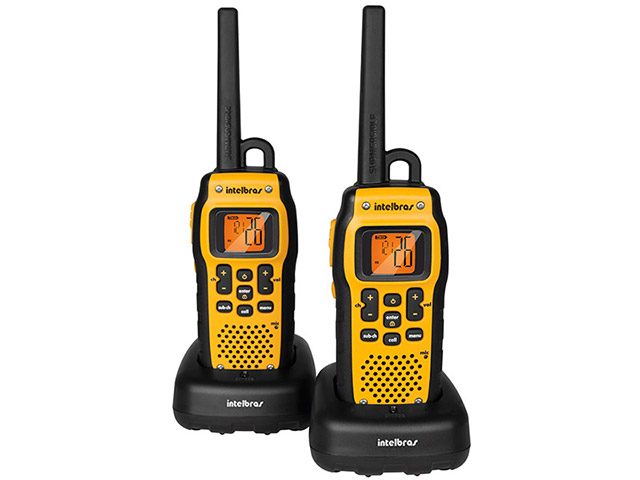
\includegraphics[keepaspectratio=true,scale=0.5]{monitoramento/radio.jpg}
	\caption{Radio comunicador para monitoramento.}
\end{figure}

\subsection{Bicicleta}

O modelo de bicicleta será a GONEW ENDORPHINE 51 com o preço unitário R\$ 584,10, (quantidade estabelecida pelo comprador do projeto). 

\begin{figure}[H]
	\centering
	\label{Bicicleta para monitoramento.}
		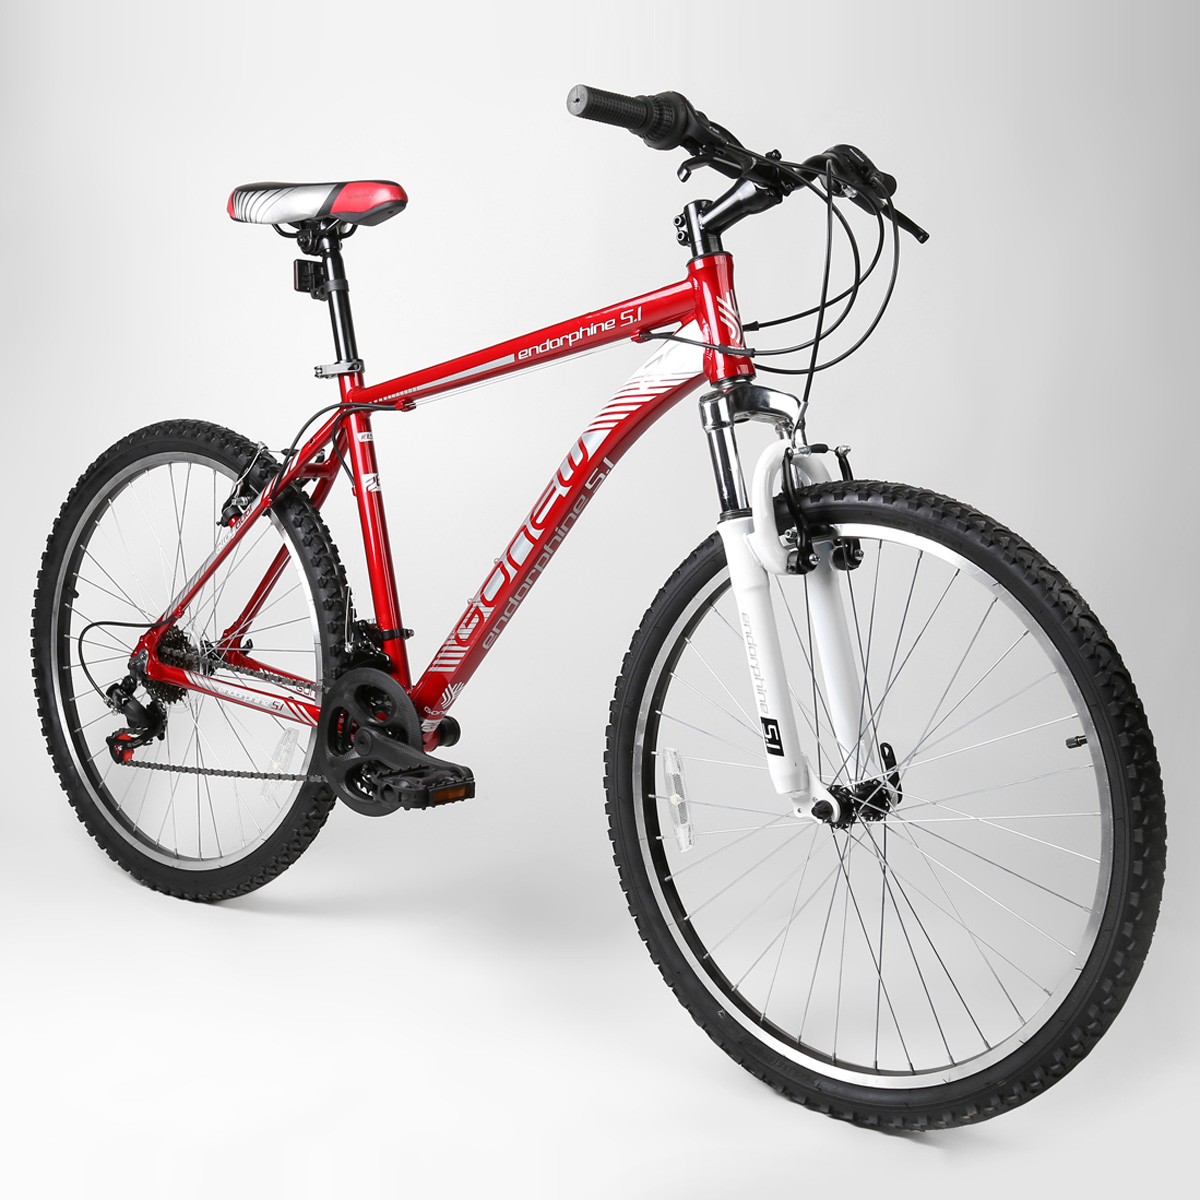
\includegraphics[keepaspectratio=true,scale=0.2]{monitoramento/Bicicleta.jpg}
	\caption{Bicicleta para monitoramento.}
\end{figure}

\subsection{Motocicleta}

\begin{figure}[H]
	\centering
	\label{Motocicleta para monitoramento.}
		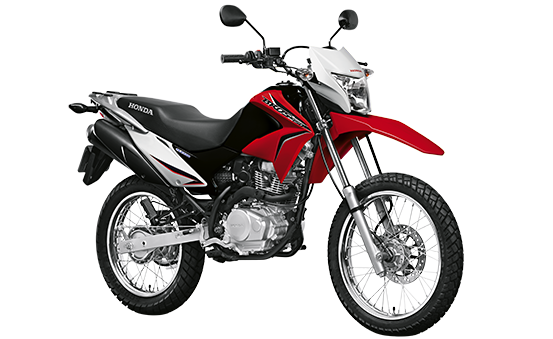
\includegraphics[keepaspectratio=true,scale=2.0]{monitoramento/Moto.png}
	\caption{Motocicleta para monitoramento.}
\end{figure}

O modelo que será utilizado é a Honda NXR 150 BROS -Figura 3- , com o preço unitário  de R\$ 9050,00.

\subsection{Consumo Energético do sistema de monitoramento}

\begin{itemize}
	\item Câmeras: 
	\begin{itemize}
	\item Potência para um elemento (hora): 15 W
 	\item Potência consumida por todas as câmeras (hora): 150 W
	\item Potência consumida por dia pelo conjunto (dia):3600 W
	\item Potência consumida mensalmente pelo conjunto: 108 kW
	\item KiloWhatt/hora(conjunto): 0.15kW/hora	
	\end{itemize}

	\item Gravador de vídeo:
	\begin{itemize}
	\item Consumo por hora: 40 W
	\item Consumo mensal: 28,8kW
	\item Kilowhat/hora: 0.04kW/h
	\end{itemize}		
	
	\item Hds:
	\begin{itemize}
	\item Consumo por hora (2 Hds):8.8 kW
	\item Cosumo mensal (2 hds): 6,336 kW
	\item KiloWhat/hora:0.0088 kW/h
	\end{itemize}

\end{itemize}

\begin{itemize}
	\item Cálculos para potência:
	\begin{itemize}
		\item Diário:
		O cálculo da potência diária é feito multiplicando a potência consumida por hora pelo número de horas que o equipamento ficará ligado. No projeto todos os equipamentos de monitoramento ficarão ligados 24 horas.
		\begin{equation}
			Potência Diária = (Potência Do Equipamento) \ast  24
		\end{equation}

		\item Mensal:
		A potência mensal é dada pela multiplicação entre potência diária vezes 30.
		\begin{equation}
			Potência Mensal =  (Potência Diária) \ast  24
		\end{equation}
		
		
		\item KW/h:
		O cálculo do KW/h é feito dividindo a potência mensal por 720, que o número de horas no mês.
		
		\begin{equation}
			Valor(\frac{kW}{h}) = (\frac{potência mensal}{720})
		\end{equation}
			
	\end{itemize}
	
	\item Cálculo do custo
	\begin{itemize}
		\item Câmeras:
   		 O cálculo do custo das câmeras foi efetuado pela multiplicação do preço unitário com o número de unidades.
		\begin{equation}
		(Número de Câmeras) \ast  (Preço Unitário)
		\end{equation}
		
		\item Hds:
  		O cálculo do custo dos hds foi feito pela multiplicação do números de  hds pelo preço unitário

		\begin{equation}
		(Número De Hds) \ast  (Preço Unitário)
		\end{equation}		 

		\item Cabos coaxiais:
		O cálculo do custo dos cabos coaxiais foi feito multiplicando a metragem total de cada setor pelo preço por metro.
		\begin{equation}
		(Metragem Requerida) \ast (Preço Por Metro)	
		\end{equation}			
	\end{itemize}
\end{itemize}

\subsection{Preço total do sistema de monitoramento}

A Tabela 20 mostra o preço total do sistema de monitoramento por câmeras, por meio do preço de cada módulo de compõe esse sistema, como elucidado na equação a seguir.

Para obtenção dos valores foi consultado o valor em 06/2015 do equipamento em lojas virtuais como simplesclique.com (Câmera), eletronicasantana.com (Gravador de vídeo), fourserv.com (Disco Rígido), fonteseg.com (Cabos), magazineluiza.com (Fonte), netshoes.com (Bicicleta), Honda.com (moto).

\begin{equation}
	\sum (Modulo Do Sistema De Monitorametno)
\end{equation}
 
\begin{table}[h]
\centering
\caption{Custo total monitoramento}
\label{Custo total monitoramento}
\begin{tabular}{llll}
 &  &  &  \\ \hline
\multicolumn{1}{|l|}{Produto} & \multicolumn{1}{l|}{Quantidade} & \multicolumn{2}{l|}{Valor R\$} \\ \hline
\multicolumn{1}{|l|}{Câmera} & \multicolumn{1}{l|}{10} & \multicolumn{2}{l|}{99244,8} \\ \hline
\multicolumn{1}{|l|}{Gravador} & \multicolumn{1}{l|}{1} & \multicolumn{2}{l|}{2029} \\ \hline
\multicolumn{1}{|l|}{HD} & \multicolumn{1}{l|}{2} & \multicolumn{2}{l|}{1371,07} \\ \hline
\multicolumn{1}{|l|}{Cabos} & \multicolumn{1}{l|}{1500(metros)} & \multicolumn{2}{l|}{4049,68} \\ \hline
\multicolumn{1}{|l|}{Radio Comunicador} & \multicolumn{1}{l|}{1 Par} & \multicolumn{2}{l|}{459} \\ \hline
\multicolumn{1}{|l|}{Bicicleta} & \multicolumn{1}{l|}{1} & \multicolumn{2}{l|}{584,1} \\ \hline
\multicolumn{1}{|l|}{Moto} & \multicolumn{1}{l|}{1} & \multicolumn{2}{l|}{9050} \\ \hline
\multicolumn{2}{|l|}{Preço Total} & \multicolumn{2}{l|}{116787,65} \\ \hline
\end{tabular}
\end{table}

\section{Balanço financeiro para a manutenção}

\subsection{Cercamento}

Primeira opção: Estoque

O técnico em eletrônica ganha em média 1000 reias

\begin{itemize}
          \item O auxiliar de manutenção no ramo de cercamento ganha em média entre 724 reais e 1124 reais mensais \cite{catho}
          \item Furadeira - Impacto profissional 3000 rpm - GSB 16 RE- 314 reais à vista
          \item Broca HSS-G 8x75x117mm Bosch- \$ 7,90 \cite{agrotama}
          \item Parafuso Madeira Cabeça Chata Latão Polido Cartela Com 10 Peças Vonder 3,2X20 Mm - 11.90 reais \cite{fixpar}
          \item Parafuso madeira fenda philips cabeça panela chip board tamnho: 4.0x50 Embalagem com 100 UNIDADES - 5.77 reais \cite{fixpar}
          \item Parafuso madeira de fenda simples cabeça chata tamanho: 6,1X90 Embalagem com 100 unidades - 22.58 reais \cite{fixpar}
\end{itemize}

	Se tratando desta opção os custos de manutenção são explicitado na tabela acima, sendo o material necessário a ser comprado inicialmente. A reposição destes materiais só ocorrerá devido a necessidade de manutenção ou quando se esgota o prazo de validade de cada elemento.
	
Segunda Opção: Contratação da empresa terceirizada.

	Já em relação a segunda opção para cercamento ficará sobre o encargo do comprador do projeto para escolher a empresa terceirizada que realizará essa atividade caso ele escolha essa opção de manutenção assim os custos de manutenção serão combinados com o comprador e a empresa no momento da contratação. Assim mandamos e-mail para fazer uma simulação da manutenção, mas infelizmente não houve resposta.
	
\subsection{Iluminação}
	
Estoque:

O auxiliar de manutenção elétrica ganha em média entre 980 reais a 1198 reais mensais \cite{catho} .
	O sistema de manutenção da iluminação ocorrerá apenas com uma vertente que é a do estoque, devido ao segredo industrial dos postes utilizados. Como o fornecimento de energia é publico então essa manutenção será realizada pelo órgão público responsável.  O estoque será realizado com os elementos relatados acima juntamente com o seu respectivo valor. Assim de maneira análoga ao cercamento esses elementos deverão ser comprados inicialmente e a reposição ocorrerá devido à necessidade de manutenção e prazo de validade do equipamento.
	
\subsection{Monitoramento}

Primeira opção: Estoque

O técnico em eletrônica ganha em média 1000 reais mensais

	Os custos desta opção serão de forma análoga ao cercamento onde inicialmente deverá comprar todos os equipamentos necessários descritos acima com o seu respectivo valor, e a reposição ocorrerá quando houver a necessidade de manutenção e o vencimento do prazo de validade do determinado equipamento.
	Em relação a motocicleta a manutenção não obedecerá ao estoque pois ficaria inviável, então quando houver a necessidade de manutenção a motocicleta será enviada para uma oficina mais próxima ou para a autorizada. Vale ressaltar o valor das revisões, ou seja, as manutenções preventivas serão:
	
Primeira revisão 1000km - 58 reias \cite{yamaha} .
Segunda revisão 5000km - 25 reais \cite{yamaha} .
Terceira revisão 10000km - 216 reais \cite{yamaha} .

	O preço da manutenção tanto na autorizada quanto na oficina dependerá da necessidade de manutenção a ser combinado com a oficina ou com a própria autorizada.
	
Segunda Opção contratação da empresa terceirizada

	Já em relação a segunda opção para monitoramento ficará sobre o encargo do comprador do projeto para escolher a empresa terceirizada que realizará essa atividade caso ele escolha essa opção de manutenção assim os custos de manutenção serão combinados com o comprador e a empresa no momento da contratação. Assim mandamos e-mail para fazer uma simulação, mas infelizmente não houve resposta.
	
\subsection{Custo final Manutenção}

	Vale ressaltar, que o valor final de manutenção está levando em conta um caso extremo, onde na pior das hipóteses supondo que todas as câmeras têm algum tipo de problema que as tornem inutilizadas, assim a manutenção seria de modo a repôr as câmeras, e o valor da manutenção seria, a soma do valor das câmeras com o valor do outros equipamentos para a manutenção do cercamento e monitoramento. Sabe-se que a iluminação não entra nessa conta, pois estamos considerando apenas o estoque. Nessas condições o valor final é de R\$ 122.690,47. Agora, se tratando de um caso mais comum onde acontece um problema na câmera e o problema será solucionado trocando apenas algum componente da mesma, esse valor de manutenção dependerá da situação e necessidade, resultando em um valor final de manutenção menor do que o considerado acima.
	
\section{Balanço financeiro para a interação social}

\subsection{Espaço Interativo}

\begin{table}[h]
\centering
\caption{Estrutura}
\label{Estrutura}
\begin{tabular}{llllllllll} \\ \hline 
Descrição                &  & Qtd. & Cor da lona     &  & (M)LxC & (M)PéDireito & (M)Metr.Total & Fech.Lateral & R\$        \\ \hline 
Galpão Modulado          &  & 1    & Branca ou Cinza &  & 40x50  & 4            & 2.000         & sim          & 439.000,00 \\ \hline 
Porta Corrediça          &  & 1    & Branca ou Cinza &  & 5      & 4            & 16            & sim          & Cortesia   \\ \hline 
Valor Total de produtos: &  &      &                 &  &        &              &               &              & 439.000,00 \\ \hline 
\end{tabular}
\end{table}

\begin{table}[h]
\centering
\caption{Despesas Operacionais}
\label{DespesasOperacionais}
\begin{tabular}{|l|l|l|l|}
\hline
Item                        & Descrição                                                       & Qtd. & R\$       \\ \hline
1                           & Frete/ Equipe técnica (montagem)                                & 1    & 12.000,00 \\ \hline
2                           & Frete/ Equipe técnica (desmontagem)                             & 0    & 0         \\ \hline
3                           & ART (Atestado de Responsabilidade Técnica - CREA SP) – Opcional & 1    & Incluso   \\ \hline
4                           & Laudo de Inflamabilidade (IPT)                                  & 1    & Incluso   \\ \hline
5                           & Outras despesas (Munck, Alimentação, Hospedagem)                & 1    & Incluso   \\ \hline
Valor Total de mobilização: &                                                                 &      & 12.000,00 \\ \hline
\end{tabular}
\end{table}

\textbf{Especificações técnicas da estrutura}

\textbf{- Lona Vinílica} - Confeccionada em tecido sintético (Lona Vinílica) TD3.000, especial para Coberturas, coberto com PVC laminado. Pigmentado em ambas as faces, black out (Filtro Solar), auto extinguível, anti mofo , anti fungos e anti raios U.V e I.V, impermeável, modelada e soldada por sistema de alta frequência nas emendas com reforço duplo nas extremidades, fixada na estrutura com cordas trançadas de polipropileno, gancho e argola.

Durabilidade e manutenção:

1. Durabilidade total do material: 5 anos pelo Fabricante.
2. Manutenção Geral: Por conta do comprador.
3. Manutenção Periódica: Por conta do comprador.
4. Manutenção Preventiva: Por conta do comprador.

\textbf{- Estrutura Metálica} -Aço Galvanizado a Fogocom perfis em Alumínio. Vão Totalmente Livres. Não necessário Fundação, uma vez que os pés podem ser apoiados no terreno original ( o mesmo deve estar compactado e nivelado).

Durabilidade e manutenção:
1. Durabilidade: Sem prazo pré-definido.
2. Manutenção Geral: Por conta do comprador.
3. Manutenção Periódica: Por conta do comprador.
4. Manutenção Preventiva: Por conta do comprador.

\textbf{- Fixação} - O sistema de fixação da base da estrutura devera ser estaqueada ou chumbada no próprio solo compactado devendo apresentar ainda um local com características amplas para a estocagem e instalação da estrutura modular do galpão.

\textbf{-Iluminação}

\begin{table}[h]
\centering
\caption{Custos da iluminação}
\label{CustosIluminacao}
\begin{tabular}{|l|l|l|l|}
\hline
Quantidade & Descrição                            & Preço unitário & Preço total  \\ \hline
80 UND     & Lampada Super LED 12W                & R\$34,00       & R\$2.720,00  \\ \hline
80 UND     & Plafon com bucal                     & R\$4,00        & R\$320,00    \\ \hline
40 UND     & Rolo de fio 10m e 2,5mm de expessura & R\$83,00       & R\$3.320,00  \\ \hline
5 UND      & Interruptor Sobrepon                 & R\$5,00        & R\$25,00     \\ \hline
10 UND     & Fita isolante                        & R\$6,00        & R\$60,00     \\ \hline
600 metros & Metalon 20X20X0.80MM                 & R\$16,81       & R\$10.086,00 \\ \hline
TOTAL R\$: &                                      &                & 16.531,00    \\ \hline
\end{tabular}
\end{table}

	Segundo cotação de mercado e pesquisa de produtos, chegou-se aos seguintes itens e valores, referidos na tabela acima. Dos materiais referidos acima, o que chama mais atenção são as lâmpadas de LED, pois com estas chegou-se a um enquadramento do conceito principal do projeto, que é sustentabilidade. No que se refere às lâmpadas, foi pautado para a escolha do tipo de lâmpada a economia e a durabilidade a longo prazo. Concluído que as lâmpadas super LED são mais indicadas, mesmo tendo um maior desembolso inicial com relação a outros modelos. As lâmpadas de LED possuem um raio de atuação de 5m, sendo necessárias 80 unidades para que haja uma iluminação eficiente. Outro fator de suma importância foi a economia gerada por mês, pois as lâmpadas de LED são muito mais eficientes do que as comuns pois produzem a mesma quantidade de luz (ou lúmen, para ser mais correto) utilizando bem menos energia. Além disso, a geração de calor durante esse processo é praticamente nula, o que ajuda na economia energética. Enquanto uma lâmpada incandesceste gasta certa de 60 W para produzir uma determinada quantia de lúmen, um conjunto de LED precisa de apenas 20 W. Outra grande vantagem das lâmpadas de LED é que elas são muito mais resistentes do que as incandescestes e florescentes.
	
\begin{table}[h]
\centering
\caption{Preços dos itens internos do Espaço Interativo}
\label{PrecoInternoEspacoInterativo}
\begin{tabular}{|l|l|l|l|l|}
\hline
Objeto                  & Marca       & Quantidade & Consumo(W)       & Preço(R\$) \\ \hline
Cadeiras e Mesas        & Bela Vista  & 400 e 100  & ---------------- & 21480      \\ \hline
Palco                   & Habitíssimo & 1(8x6x1)   & ---------------- & 30000      \\ \hline
Projetor                & Extra       & 1          & 280              & 4684,29    \\ \hline
Mesa de Som             & Contato Pro & 1          & 50               & 2537       \\ \hline
Amplificadores de palco & Contato Pro & 2          & 300              & 3499,8     \\ \hline
Amplificadores ambiente & Contato Pro & 20         & 1600             & 13798      \\ \hline
Total R\$:              &             &            &                  & 75999,09   \\ \hline
\end{tabular}
\end{table}

	As cadeiras e mesas com melhor custo benefício encontradas foram da marca Bela Vista, os outros orçamentos feitos com mesas e cadeiras com a mesma qualidade eram acima de R\$ 22000 reais sem frete e estas compradas pelo site restauranteshop.com.br, seriam compradas por R\$ 21480 reais com frete.
	
	Projetor BenQ MX822ST com alta qualidade de imagem com 1200 lúmens e consumo de 280 W.
	
	Para o sistema de som foram escolhidos os seguintes equipamentos: Mesa BEHRINGER – EURODESK SX2442 FX com um consumo de 50W, 2 caixas ativa ANTERA – SC10A com consumo de 150W por caixa de som e  20 caixas passiva SELENIUM – C321P com um consumo máximo de 80W por caixa.
	
	Funcionamento do espaço interativo de 10 horas por dia.
	Consumo de energia do sistema de som: 10h x 1950W X 30dias = 585kWh/mês.
	
\begin{table}[h]
\centering
\caption{Custos e consumos da bicicleta ergométrica}
\label{CustosBicicletaErgometrica}
\begin{tabular}{|l|l|l|l|l|l|}
\hline
Objeto             & Marca                    & Fornecedor     & Quantidade & Consumo(W)           & Preço Total(R\$) \\ \hline
Bicicleta(aro 24)  & Verden Live              & Buscapé        & 10         & -------------------  & 3.112            \\ \hline
Bicicleta(aro 26)  & Foxer Hammer             & Ricado Eletro  & 20         & -------------------  & 6.980            \\ \hline
Pneus (aro 26)     & Praieiro Slick - Levorin & Cia doPedal    & 40         & ------------------   & 1.240            \\ \hline
Pneus (aro 24)     & Slick Flame              & Cia da Bike    & 20         & ------------------   & 859,6            \\ \hline
Gerador            & Generator Friction       & Eletric Pedals & 30         & 12000                & 90.000,00        \\ \hline
Distribuidor       & Bus Board                & Eletric Pedals & 15         & -------------------- & 75.000,00        \\ \hline
Estação de energia & Power Station Quartk     & Eletric Pedals & 1          & 4000                 & 150.000,00       \\ \hline
Total R\$:         &                          &                &            &                      & 327.191,60       \\ \hline
\end{tabular}
\end{table}

	O gerador escolhido foi o da \textit{Eletric Pedals}, porque foi o mais completo, de baixo custo (R\$ 3.000,00) e eficiente encontrado, sua produção fornecida pela empresa é de 400 W máximo por bicicleta e médio foi de 2400 W, totalizando uma produção de 12000W/dia.
	A estação de energia escolhida foi também da \textit{Eletric Pedals}, que possui um consumo contínuo de 2000W, mas o seu pico de consumo é de 4000W, com um valor de R\$ 150.000,00.
	O distribuidor escolhido também foi da \textit{Eletric Pedals}, com um preço de R\$ 5.000,00 por aparelho. Ele funciona como uma placa de suporte para as bicicletas, com toda a fiação no interior da placa, para prevenir acidentes.
	O projeto contará com dois modelos de bicicleta, vinte de aro vinte e seis e dez de aro vinte e quatro. Com marcas distintas e preços também, respectivamente R\$ 349,00 e R\$ 311,20.
	As bicicletas escolhidas possuem pneus inadequados, por isso pneus adequados irão ser instalados.
	
\textbf{Balanço energético}

	Funcionamento do espaço interativo, juntamente com as bicicletas ergométricas de 10 horas por dia.
             As 10 horas de produção de energia através das bicicletas, serão dividas em 4 horas no período da manhã, 4 horas no período da tarde, e 2 horas no período noturno. 
             Segundo as tarifas da CEB, o valor do kWh é aproximadamente R\$1.419875.
             Produção de energia através da bicicleta: 10h x 400W x 30dias = 120.000Wh/mês.
             Calculando a economia gerada: 120kWh/mês x R\$ 1.419875 = R\$ 137,00/mês.
             
\textbf{Wi-Fi do parque}

	A tabela a seguir mostra o valor do roteador da Mikrotik que será usado nos quiosques do Parque Vivencial do Gama, mostra também o valor por unidade, o consumo de cada unidade e o valor total dos aparelhos. Ao todo serão três roteadores, um para cada quiosque.
	
\begin{table}[h]
\centering
\caption{Preços do sistema de Wi-Fi do parque}
\label{precosWiFi}
\begin{tabular}{|l|l|l|l|l|l|}
\hline
Produto                   & Fornecedor & Valor/unidade (R\$) & Consumo/unidade (W) & Quantidade & Valor total (R\$) \\ \hline
Mikrotik Routerboard 1100 & Nr Store   & 1.539,20            & 25                  & 3          & 4.617,60          \\ \hline
\end{tabular}
\end{table}

\textbf{Aplicativo do parque}

	A tabela contém o valor estimado para o desenvolvimento do aplicativo. O preço baseia-se nas pesquisas de mercado feitas para aplicativos de \textit{smartphone} e \textit{tablet} com esse grau de desenvolvimento.
	
\begin{table}[h]
\centering
\caption{Preço para desenvolvimento do Aplicativo do parque}
\label{precoAplicativo}
\begin{tabular}{|l|l|l|l|}
\hline
Produto                          & Valor (R\$) & Quantidade & Valor total (R\$) \\ \hline
Aplicativo Parque Vivencial Gama & 19.000,00   & 1          & 19.000,00         \\ \hline
\end{tabular}
\end{table}
